\documentclass[twoside,openright,titlepage,fleqn,
	headinclude,11pt,a4paper,BCOR5mm,footinclude
	]{scrbook}
%--------------------------------------------------------------
        \newcommand{\myTitle}{Analisi di reti metaboliche basata su
          propriet\`a di connessione\xspace}
% use the right myDegree option
\newcommand{\myDegree}{Corso di Laurea in Informatica\xspace}
%\newcommand{\myDegree}{
	%Corso di Laurea Specialistica in Scienze e Tecnologie 
	%dell'Informazione\xspace}
\newcommand{\myName}{Massimo Nocentini\xspace}
\newcommand{\myProf}{Pierluigi Crescenzi\xspace}
\newcommand{\myOtherProf}{Nome Cognome\xspace}
\newcommand{\mySupervisor}{Nome Cognome\xspace}
\newcommand{\myFaculty}{
	Facolt\`a di Scienze Matematiche, Fisiche e Naturali\xspace}
\newcommand{\myDepartment}{
	Dipartimento di Sistemi e Informatica\xspace}
\newcommand{\myUni}{\protect{
	Universit\`a degli Studi di Firenze}\xspace}
\newcommand{\myLocation}{Firenze\xspace}
\newcommand{\myTime}{Anno Accademico 2010-2011\xspace}
\newcommand{\myVersion}{Version 0.1\xspace}
%--------------------------------------------------------------
\usepackage[latin1]{inputenc} 
\usepackage[T1]{fontenc} 
\usepackage[square,numbers]{natbib} 
\usepackage[fleqn]{amsmath}  
\usepackage[italian]{babel}
%--------------------------------------------------------------
\usepackage{dia-classicthesis-ldpkg} 
%--------------------------------------------------------------
% Options for classicthesis.sty:
% tocaligned eulerchapternumbers drafting linedheaders 
% listsseparated subfig nochapters beramono eulermath parts 
% minionpro pdfspacing
\usepackage[eulerchapternumbers,subfig,beramono,eulermath,
	parts]{classicthesis}
%--------------------------------------------------------------
\newlength{\abcd} % for ab..z string length calculation
% how all the floats will be aligned
\newcommand{\myfloatalign}{\centering} 
\setlength{\extrarowheight}{3pt} % increase table row height
\captionsetup{format=hang,font=small}
%--------------------------------------------------------------
% Layout setting
%--------------------------------------------------------------
\usepackage{geometry}
\geometry{
	a4paper,
	ignoremp,
	bindingoffset = 1cm, 
	textwidth     = 13.5cm,
	textheight    = 21.5cm,
	lmargin       = 3.5cm, % left margin
	tmargin       = 4cm    % top margin 
}
%--------------------------------------------------------------
\usepackage{listings}
\usepackage{hyperref}
% My Theorem
\newtheorem{oss}{Observation}[section]
\newtheorem{exercise}{Exercise}[section]
\newtheorem{thm}{Theorem}[section]
\newtheorem{cor}[thm]{Corollary}

\newtheorem{lem}[thm]{Lemma}

\newcommand{\vect}[1]{\boldsymbol{#1}}

% questo comando e' relativo alle correzioni che puo
% apportare il prof se lo desidera.
\newcommand{\prof}[1]{\boldsymbol{#1}}

% instead of boldsymbol I can use the arrow above the letter with
%\newcommand{\vect}[1]{\vec{#1}}

% page settings
% \pagestyle{headings}
%--------------------------------------------------------------
\begin{document}
\frenchspacing
\raggedbottom
\pagenumbering{roman}
\pagestyle{plain}
%--------------------------------------------------------------
% Frontmatter
%--------------------------------------------------------------
%--------------------------------------------------------------
% titlepage.tex (use thesis.tex as main file)
%--------------------------------------------------------------
\begin{titlepage}
	\begin{center}
   	\large
      \hfill
      \vfill
      \begingroup
			\spacedallcaps{\myUni} \\ 
			\myFaculty \\
			\myDegree \\ 
			\vspace{0.5cm}
         
\includegraphics[scale=.065]{logo/unifi}\\
         \vspace{0.5cm}    
         Tesi di Laurea    
      \endgroup 
      \vfill 
      \begingroup
      	\color{Maroon}\spacedallcaps{\myTitle} \\ \bigskip
      \endgroup
      \spacedlowsmallcaps{\myName}
      \vfill  
      Relatore: \itshape{\myProf}
      \vfill                   
      \myTime
      \vfill                      
	\end{center}        
\end{titlepage}   
%--------------------------------------------------------------
% back titlepage
%--------------------------------------------------------------
   \newpage
	\thispagestyle{empty}
	\hfill
	\vfill
	\noindent\myName: 
	\textit{\myTitle,} 
	\myDegree, \textcopyright\ \myTime
%--------------------------------------------------------------
% back titlepage end
%--------------------------------------------------------------
\pagestyle{scrheadings}
%--------------------------------------------------------------
% Mainmatter
%--------------------------------------------------------------
\pagenumbering{arabic}

% settings for the lstlisting environment
\lstset{
	language = java
	, numbers = left 
	, basicstyle=\sffamily%\footnotesize
	%, frame=single
	, tabsize=2
	, captionpos=b
	, breaklines=true
	, showspaces=false
	, showstringspaces=false
}

\tableofcontents

% \newpage

\section*{Licenze}

Solo questa sezione dedicata alle licenze verr\`a scritta completamente in
inglese.

\subsection*{Text contents}
All the text content is distributed under:\\
\textbf{
This work is licensed under the Creative Commons
Attribution-NonCommercial-ShareAlike 3.0 Unported License. To view a copy of 
this license, visit
\\http://creativecommons.org/licenses/by-nc-sa/3.0/  or send a
letter to Creative Commons, 444 Castro Street, Suite 900, Mountain View, 
California, 94041, USA.} 


% \begin{figure}[!htb]
%  \centering
%   \includegraphics[scale=1]
%   {cc-icons-eps/by.eps}
% \end{figure}

\begin{center}

\includegraphics{cc-icons-eps/by}

\includegraphics{cc-icons-eps/cc}

\includegraphics{cc-icons-eps/nc}

\includegraphics{cc-icons-eps/sa}
\end{center}

\subsection*{Java sources}
All the Java sources are distributed under, where the word ``Software'' is
referred to all of the sources that are present in this work: \\
\textbf{
Copyright (c) 2011 Massimo Nocentini\\
Permission is hereby granted, free of charge, to any person obtaining a copy of
this software and associated documentation files (the "Software"), to deal in 
the Software without restriction, including without limitation the rights to 
use, copy, modify, merge, publish, distribute, sublicense, and/or sell 
copies of the Software, and to permit persons to whom the Software is furnished 
to do so, subject to the following conditions:\\
The above copyright notice and this permission notice shall be included in all 
copies or substantial portions of the Software.\\
THE SOFTWARE IS PROVIDED "AS IS", WITHOUT WARRANTY OF ANY KIND, EXPRESS OR 
IMPLIED, INCLUDING BUT NOT LIMITED TO THE WARRANTIES OF MERCHANTABILITY, 
FITNESS FOR A PARTICULAR PURPOSE AND NONINFRINGEMENT. IN NO EVENT SHALL THE 
AUTHORS OR COPYRIGHT HOLDERS BE LIABLE FOR ANY CLAIM, DAMAGES OR OTHER LIABILITY, 
WHETHER IN AN ACTION OF CONTRACT, TORT OR OTHERWISE, ARISING FROM, OUT OF OR IN 
CONNECTION WITH THE SOFTWARE OR THE USE OR OTHER DEALINGS IN THE SOFTWARE.
}


% \newpage
% \section*{Sinopsi}

% \newpage
% 
\section*{Syntax and Format}

Nel documento i termini \emph{vertice} e \emph{nodo} sono da
considerarsi equivalenti e per questo verranno utilizzati in modo
interscambiabile.

\section*{Used Tools}

\newpage
\chapter{Introduzione}
\label{chapter:introduction}
Questo lavoro ha come obiettivo l'analisi di reti metaboliche:
cercheremo di astrarre i processi fisici che avvengono all'interno
delle cellule di organismi, utilizzando la struttura astratta grafo in
modo da poter ragionare su quest'ultimo utilizzando algoritmi ben noti
della teoria dei grafi. In particolare indagheremo la relazione di
connessione forte, ricercando le componenti fortemente connesse.
\\\\
In questo capitolo si definisce cosa sono le reti metaboliche, il
motivo per cui vengono studiate, come formulare un modello astratto
che descriva una rete, quali sono i risultati gi\`a noti che
condividono alcuni aspetti di questo lavoro e quali sono gli obiettivi
che vogliamo raggiungere.

% Numerosi sistemi biologici possono essere modellati con il concetto
% astratto di grafo. Studiare la struttura e la topologia di
% quest'astrazione non fornisce solo una descrizione dei complessi
% comportamenti del sistema in oggetto ma, pu\`o essere di grande
% utilit\`a per capire le funzionalit\`a del sistema e le sue dinamiche.

% Inoltre attraverso questo processo di astrazione, \`e possibile
% studiare quali relazioni possono intercorrere tra il sistema e il
% contesto che lo ospita. Lo studio di queste relazioni pu\`o portare a
% fare delle stime riguardo la potenzialit\`a del sistema di
% ``comunicare'' con il contesto.

% Le idee che abbiamo espresso sono alla base del concetto di
% \emph{storia} che avremo modo di studiare meglio nel Capitolo
% \ref{chapter:theoretical-background}.  

\section{Enzimi, cammini e reti metaboliche}

Prima di dare la definizione di \emph{rete metabolica} introduciamo i
concetti di cammino metabolico, enzima e da cosa \`e caratterizzata
una reazione chimica.

Un \emph{cammino metabolico} \`e una sequenza di reazioni chimiche che
si verificano all'interno di una cellula. Dal punto di vista
matematico, possiamo vedere un cammino metabolico come una sequenza di
funzioni, dette reazioni, che, avendo in input un insieme di molecole,
esegue delle trasformazioni su queste e produce come output il
risultato delle trasformazioni svolte, sotto forma di insieme di
molecole. Questo output pu\`o essere utilizzato come input per la
funzione successiva, concatenando quanto si voglia le trasformazioni.

Ogni reazione chimica \`e regolata da alcuni \emph{enzimi}. Un
\emph{enzima} \`e una proteina che gestisce la frequenza e la
velocit\`a di una reazione chimica. Le molecole a cui si applica la
reazione vengono identificate con il termine \emph{substrato} (o
\emph{reagenti}), mentre le molecole output della reazione vengono
identificate con il termine \emph{prodotti}.  Durante l'esecuzione di
una reazione chimica, ogni enzima agisce da \emph{catalizzatore},
ovvero non viene consumato nella reazione e, quindi, pu\`o partecipare
in pi\`u di una reazione.

L'insieme di enzimi ``guida'' e determina l'insieme di cammini
metabolici che possono occorrere nella cellula, in quanto una reazione
chimica su un substrato pu\`o avvenire se e solo se lo strato attivo
del substrato \`e complementare allo strato attivo dell'enzima.
\\\\
Adesso possiamo definire una \emph{rete metabolica} come collezione di
cammini metabolici. Le reti metaboliche sono ampiamente studiate in
quanto caratterizzano le propriet\`a fisiologiche e biochimiche delle
cellule. Analizzare queste reti permette la ricostruzione delle
reazioni biochimiche che avvengono all'interno di molti organismi, sia
questi batteri che esseri umani.
\\\\
Nelle prossime sezioni studieremo un linguaggio che permetta di
codificare le reti metaboliche, descrivendo in particolare i concetti
necessari al nostro lavoro.

\section{Il linguaggio SBML}
\textbf{SBML} (\textbf{S}ystems \textbf{B}iology \textbf{M}arkup
\textbf{L}anguage) \`e un linguaggio che permette di rappresentare
informazioni classificandole in modo gerarchico, basato sul linguaggio
XML.

SBML \`e orientato alla descrizione di sistemi in cui entit\`a
biologiche sono oggetto di manipolazioni eseguite da processi nel
corso del tempo e, pertanto, facilita la codifica di modelli
computazionali di processi biologici, come, ad esempio reti
metaboliche, segnalazioni cellulari e molti altri.

Nel seguito, dopo aver formalizzato un sistema con questo linguaggio,
faremo riferimento a tale formalizzazione con il termine ``modello
SBML'' del sistema in questione.

\subsection{Oggetti e propriet\`a fondamentali}
\label{sec:necessaryRealObjectsModeledInSBML}

Nella precedente sezione abbiamo introdotto, per inquadrare il
problema, alcuni concetti che non sono influenti sul nostro studio: in
questa sezione trattiamo solo quelli inerenti al lavoro che abbiamo
sviluppato, nonostante molti dei concetti non usati siano modellabili
con SBML.
\\\\
L'unit\`a atomica definibile con SBML \`e il \emph{metabolito}, che
rappresenta il concetto di molecola.  Un oggetto di questo tipo ha
molti attributi ma, ai nostri fini, tre sono quelli necessari:
\begin{description}
\item[identificatore] rappresentato da un'etichetta, univoca in tutto
  il modello, permette di distinguerlo dagli altri metaboliti;
\item[nome] rappresentato da un'etichetta, possibilmente non univoca,
  permette di associargli delle informazioni di pi\`u alto livello
  rispetto all'\emph{identificatore};
\item[compartimento] rappresentato da un'etichetta, univoca in tutto
  il modello, permette di associargli il compartimento della cellula
  dove risiede (in tutti gli esempi che abbiamo avuto modo di testare
  il compartimento \`e sempre il \emph{citoplasma}).
\end{description}

Un altro concetto fondamentale \`e quello di \emph{reazione chimica},
codificato in SBML con:
\begin{description}
\item[reagenti] insieme di \emph{metaboliti}, modella il
  substrato della reazione;
\item[prodotti] insieme di \emph{metaboliti}, modella i
  prodotti della reazione;
\item[reversibile] valore booleano, specifica se la reazione \`e
  reversibile oppure no.
\end{description}
Questo \`e quello che ci serve per iniziare ad analizzare il modello
SBML di un organismo: ricercheremo l'insieme di reazioni descritte e,
per ogni reazione, analizzeremo l'insieme dei \emph{reagenti} e dei
\emph{prodotti} per costruire un grafo oggetto dei nostri studi. Nella
prossima sezione descriveremo le regole che abbiamo utilizzato per
costruirlo.

\subsection{Costruire un grafo da un modello SBML}

Non \`e possibile utilizzare direttamente i concetti espressi con il
linguaggio SBML come input per i nostri algoritmi, dobbiamo prima
trasportarli in una struttura dati grafo. Questo passaggio ci permette
di ridurre la complessit\`a e la mole delle informazioni, riducendo il
problema originale ad un problema a cui \`e possibile applicare
algoritmi appartenenti alla teoria dei grafi.

In particolare, il grafo che costruiremo \`e un grafo orientato, la
cui caratteristica \`e quella di partizionare l'insieme dei vertici in
due partizioni. Identificheremo i vertici a seconda della partizione
di appartenenza come vertici \emph{neri} o \emph{bianchi} (vedi
\cite{tellingStories}).
\\\\
Per costruire il grafo usiamo questo insieme di regole:
\begin{itemize}
\item due specie sono uguali se hanno uguale identificatore ed uguale
  compartimento. Questa regola \`e necessaria per evitare
  un'esplosione del numero di vertici in quanto, date due reazioni $r,
  r'$ e due metaboliti $a, a'$ tali che $a \in reagenti(r) \wedge a'
  \in reagenti(r')$, con $a = a' \wedge r \not = r'$, se si
  costruissero due nodi distinti rispettivamente per $a$ e $a'$ il
  grafo non avrebbe informazioni significative, perch\'e degenererebbe
  ad un insieme di sotto grafi isolati, ognuno rappresentante una
  reazione. Da questo segue che un metabolito non \`e identificato
  dalle reazioni in cui appare;
\item data una reazione non reversibile $r$ tale che:
  \begin{displaymath}
    \begin{split} 
      reagenti(r) &= \{ r_{1}, \ldots, r_{n} \} \\
      prodotti(r) &= \{ p_{1}, \ldots, p_{m} \}
    \end{split}
  \end{displaymath}
  allora costruiremo il grafo che codifica la relazione $reagenti(r)
  \times prodotti(r)$. Ad esempio, con $reagenti(r) = \{ a, b, c, d
  \}$ e $prodotti(r) = \{a, e, f\}$ otteniamo il grafo riportato in
  Figura \ref{fig:non-reversible-reaction-mapping};
  \begin{figure}
    \centering
    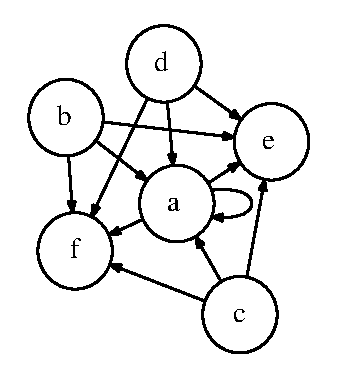
\includegraphics{images/non-reversible-reaction-example.dot.eps}
    \caption{Grafo ottenuto da una reazione non reversibile}
    \label{fig:non-reversible-reaction-mapping}
  \end{figure}
\item data una reazione reversibile $r$ tale che:
  \begin{displaymath}
    \begin{split} 
      reagenti(r) &= \{ r_{1}, \ldots, r_{n} \} \\
      prodotti(r) &= \{ p_{1}, \ldots, p_{m} \}
    \end{split}
  \end{displaymath}
  allora costruiremo il grafo che codifica la relazione $(reagenti(r)
  \times prodotti(r)) \cup (prodotti(r) \times reagenti(r))$. Ad
  esempio, con $reagenti(r) = \{ a, b, c, d \}$ e $prodotti(r) = \{a,
  e, f\}$ otteniamo il grafo riportato in Figura
  \ref{fig:reversible-reaction-mapping}.
  \begin{figure}
    \centering
    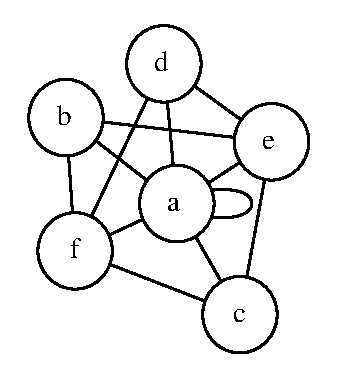
\includegraphics{images/reversible-reaction-example.dot.eps}
    \caption{Grafo ottenuto da una reazione reversibile}
    \label{fig:reversible-reaction-mapping}
  \end{figure}
\end{itemize}
Le regole descritte sopra pongono dei limiti sulle informazioni che si
codificano nel grafo finale. Per esempio tutti gli attributi delle
reazioni descritti in SBML vengono ignorati. Questo non rende
insufficiente la nostra rappresentazione in quanto miriamo alla
relazione di connessione estratta delle reazioni e non a loro
particolari propriet\`a.

Dobbiamo essere coscienti che applicando le precedenti regole facciamo
un passo di astrazione che comporta della perdita di precisione: nel
risultante grafo avremo codificato per ogni metabolito l'insieme di
metaboliti in cui questo pu\`o essere trasformato, a prescindere dalle
particolari reazioni che definiscono le trasformazioni.

\section{Riferimenti a lavori esistenti}
Il lavoro esposto in \cite{large-scale-reconstruction} ha come
obiettivo lo studio di reti metaboliche per identificare quelli che
vengono chiamati nell'articolo originale \emph{seed sets}: questi
rappresentano degli insiemi di molecole che sono delle ``interfacce''
tra la rete metabolica e il contesto che la ospita. Una volta
identificati questi insiemi, si procede ad analizzarli e trarre
conclusioni di natura biologica.

Abbiamo citato questo lavoro in quanto condivide parte del processo di
astrazione della rete e l'applicazione di algoritmi con il presente
documento.
\\\\
Il nostro lavoro ha come obiettivo di essere d'ausilio al lavoro
esposto in \cite{tellingStories}, che studia una variante del problema
di enumerare tutti i sotto grafi aciclici di un grafo orientato,
aggiungendo il vincolo che solo un determinato sottoinsieme
$\mathbb{B}$ di vertici possono avere il ruolo di sorgente o di pozzo
nei \emph{DAG} enumerati. Ogni \emph{DAG} che soddisfa tale condizione
\`e chiamato \emph{storia} e si vuole ``raccontare'' tutte le
possibili storie dato un grafo orientato e l'insieme
$\mathbb{B}$. Ricordiamo che un \emph{DAG} \`e un grafo orientato che
non contiene cicli.

\section{Nostri obiettivi}
Il concetto catturato dall'insieme $\mathbb{B}$, introdotto nella
precedente sezione, \`e quello di definire il ruolo che alcuni vertici
``interpreteranno'' nella \emph{storia} (se $v \in \mathbb{B}$ allora
$v$ avr\`a il ruolo di \emph{sorgente} o \emph{pozzo}, altrimenti il
ruolo di \emph{intermedio}).

Attualmente l'insieme $\mathbb{B}$ viene costruito in base a
osservazioni e studi \emph{empirici}, ed \`e costituito dall'insieme
di metaboliti che hanno particolari propriet\`a in determinate
condizioni.  Ci chiediamo se \`e possibile identificare l'insieme
$\mathbb{B}$ in modo automatico per analizzare la rete metabolica
utilizzando gli algoritmi esposti in \cite{tellingStories}.
\\\\
Per rispondere a tale domanda abbiamo deciso di analizzare la
connettivit\`a del grafo in input, ricercando le sue componenti
fortemente connesse. Questa idea si basa sulle seguenti motivazioni:
\begin{itemize}
\item \`e difficile cercare di assegnare il ruolo ad ogni vertice
  studiando l'istanza completa del grafo in input, in quanto astrarre
  una rete metabolica comporta grafi con molti vertici e numerosi
  archi ed, inoltre, possono esistere (con molta frequenza) cicli che
  portano solo ridondanza e complessit\`a, che quindi possiamo
  escludere in quanto non aggiungono informazioni.

  Identificando invece la decomposizione in componenti fortemente
  connesse, \`e possibile astrarre dai cicli ed identificare classi di
  metaboliti equivalenti che possono essere visti come uno solo;
\item come vedremo nella Sezione \ref{subsection:some-definitions},
  ogni componente fortemente connessa \`e una classe di equivalenza
  della relazione di connessione forte. 

  Ci\`o significa che due metaboliti appartenenti alla stessa
  componente fortemente connessa possono essere ottenuti l'uno
  dall'altro, attraverso una catena di reazioni nella rete metabolica
  che stiamo analizzando. Possiamo quindi associare a questi
  metaboliti lo stesso ruolo che viene associato alla componente che
  li contiene;
\item il ``meta grafo'' che ha come vertici le componenti fortemente
  connesse e come archi gli archi che collegano metaboliti contenuti
  in componenti diverse (evitando duplicazioni), permette di assegnare
  alle componenti un ruolo. Se una componente \`e \emph{sorgente} o
  \emph{pozzo} nel meta grafo allora possiamo inserire i vertici che
  la compongono nell'insieme $\mathbb{B}$.
\end{itemize}
Utilizzando quanto detto sopra procederemo ad applicare al grafo in
input l'algoritmo di Tarjan (in realt\`a la variante descritta nella
Sezione \ref{subsection:crescenzi-gambosi-grossi}), determineremo il
ruolo delle componenti e, di conseguenza, sar\`a possibile assegnare
un ruolo anche ai vertici.
\\\\
Per automatizzare tutte le idee esposte nei paragrafi precedenti
abbiamo prodotto una libreria Java nella quale vengono implementati i
concetti esposti nel Capitolo
\ref{chapter:theoretical-background}. Questa libreria non \`e
orientata ad essere utilizzata come un programma a se stante, bens\`i
mira ad un utilizzo programmatico ed estendibile. Per questo motivo
abbiamo ritenuto opportuno riportare nella Sezione
\ref{section:packages-descriptions} una descrizione di ogni
\emph{pacchetto} in modo da favorirne la comprensione e l'utilizzo.

Nella libreria \`e presente anche una maschera realizzata utilizzando
il framework \emph{SWING} per la renderizzazione di un particolare
insieme di risultati, relativi alla composizione delle componenti
fortemente connesse: questo \`e l'unico oggetto che non \`e possibile
utilizzare programmaticamente.

\section{Sinopsi}
In questa sezione elenchiamo i capitoli in cui questo documento \`e
suddiviso e, per ognuno di essi, daremo una breve descrizione del
contenuto.

Questo capitolo contiene un'introduzione al lavoro svolto.

Il Capitolo \ref{chapter:theoretical-background} modella da un punto
di vista teorico i concetti e gli algoritmi alla base delle
implementazioni, in particolare cosa significa visitare un grafo,
approfondiremo la strategia \emph{Depth First} e studieremo tre
algoritmi per la ricerca delle componenti fortemente connesse.

Il Capitolo \ref{chapter:study} formalizza gli obiettivi che vogliamo
raggiungere con lo sviluppo della libreria Java. Vengono proposti i
casi d'uso che abbiamo implementato e, per ognuno di essi, vengono
riportati degli esempi del ``prodotto finito'' in modo da visualizzare
i risultati se non si \`e avuto modo di utilizzare la
libreria. Inoltre si analizza l'architettura che caratterizza l'intera
implementazione.

Il Capitolo \ref{chapter:implementation} affronta tutte le questioni
inerenti alla fase di implementazione. Si discute la metodologia di
sviluppo utilizzata, alcuni paradigmi e idiomi usati ripetutamente
durante la fase di codifica ed una breve descrizione dei
\emph{pacchetti} che compongono il progetto.

Il Capitolo \ref{chapter:conclusions} termina il lavoro esponendo i
risultati ottenuti ed elencando una lista di sviluppi futuri del
progetto.

\section{Strumenti utilizzati}
Per lo sviluppo di questo progetto sono stati utilizzati i seguenti
strumenti:
\begin{itemize}
\item per la stesura di questo documento \`e stato usato il motore di
  formattazione \TeX, utilizzando \emph{Emacs} come editor dei file
  sorgenti, installando la \emph{major mode AucTex};
\item l'implementazione della libreria Java \`e stata sviluppata
  completamente con \emph{Eclipse} versione \emph{Indigo}. La JVM
  utilizzata per lo sviluppo \`e quella fornita da \emph{openjdk-6
    (versione 24)};
\item i sorgenti, sia dell'elaborato testuale sia
  dell'implementazione, sono stati versionati utilizzando il sistema
  \emph{Git}. Abbiamo utilizzato \emph{Github} come fornitore del
  servizio. I sorgenti di questo documento possono essere scaricati
  dall'URL:\\
  \href{https://github.com/massimo-nocentini/my-undergraduate-thesis}{
    https://github.com/massimo-nocentini/my-undergraduate-thesis}\\
  mentre i sorgenti dell'implementazione Java dall'URL:\\
  \href{https://github.com/massimo-nocentini/my-undergraduatethesis-java}{
    https://github.com/massimo-nocentini/my-undergraduatethesis-java}
\end{itemize}

\section{"Telling stories" characterization}
Il concetto di \emph{story} viene introdotto nell'articolo
\footnote{aggiungere qui riferimento bibliografico all'articolo di
  Crescenzi-Marino}. Prima di dare la definizione di tale concetto e
vederne un esempio, procediamo con ordine descrivendo il contesto che
ha portato alla sua formalizzazione.
\\\\
Il problema oggetto dell'articolo \`e quello di studiare una variante
del problema di enumerare tutti i sottografi di un grafo orientato in
input: tali sottografi devono essere aciclici (dei \emph{DAG}) e
massimali.

La caratterizzazione aggiuntiva che si considera \`e che solo un
determinato sottoinsieme $\mathbb{B}$ di nodi possono avere il ruolo
di sorgente o di pozzo nei \emph{DAG} che verranno enumerati. 

Questo ulteriore vincolo nasce da dalle questioni biologiche come
abbiamo analizzato nella sezione \footnote{aggiungere qui riferimento
  alla sezione che ancora devo scrivere nell'introduzione che spiega
  il contesto biologico.}. Attualmente l'insieme $\mathbb{B}$ viene
costruito in base a delle osservazioni e studi \emph{empirici},
costituito da tutte quelle \emph{species} che hanno una particolare
frequenza di produzione \footnote{chiedere se \`e corretto
  interpretare in questo modo} in determinate condizioni.

Siamo interessati ad individuare le reazioni che possono svilupparsi
da \emph{species} appartenenti all'insieme $\mathbb{B}$, studiando
percorsi nel grafo che non comportano cicli (ecco la richiesta che i
sottografi enumerati devono essere \emph{DAG}) e che allo stesso tempo
attraversino il maggior numero di \emph{species} (la richiesta di
massimalit\`a). Questi percorsi (o reazioni che dir si voglia) possono
attraversare \emph{species} che non appartengono all'insieme
$\mathbb{B}$, basta che la \emph{species} in cui inizia il percorso e
quella in cui esso termina, vi appartengano. Un sottografo che cattura
un insieme di percorsi che soddisfano le queste richieste viene
definito \emph{story}.

Il problema di fondo trattato dall'articolo \footnote{aggiungere qui
  riferimento bibliografico sempre al relativo articolo} \`e quello di
"raccontare" tutte le possibili storie dato un grafo orientato in
input e il sottoinsieme di vertici $\mathbb{B}$.

\section{Who knows about $\mathbb{B}$?}
Come abbiamo visto nella precedente sezione, l'insieme $\mathbb{B}$
viene costruito dopo studi \emph{empirici}. Il concetto catturato da
questo insieme \`e quello di definire il "ruolo" da attribuire ad
alcuni vertici che dovranno "interpretare" nella \emph{story} (se $v
\in \mathbb{B}$ allora avr\`a il ruolo di \emph{sorgente} o
\emph{pozzo}, altrimenti il ruolo di \emph{intermedio}).

Ci chiediamo se l'identificazione di tale insieme \`e possibile
effettuarla in modo automatico, utilizzando una macchina. Questo \`e
lo scopo del presente lavoro.
\\\\
Per rispondere a tale domanda vogliamo analizzare la struttura del
grafo in input dal punto di vista delle sue strongly connected
components. Questa idea si base sulle seguenti motivazioni:
\begin{itemize}
\item \`e difficile cercare di assegnare il ruolo ad ogni vertice
  studiando l'istanza completa del grafo in input, in quanto oltre ai
  percorsi a cui siamo interessati nel modello di \emph{story},
  possono esistere (e con molta frequenza) cicli che portano solo
  ridondanza e complessit\`a, che quindi possiamo escludere in quanto
  non portano informazioni aggiuntive. 

  Identificando invece la decompisizione in strongly connected
  components, \`e possibile astrarre dai cicli e trattare tutte quelle
  \emph{species} "equivalenti" (vedi prossimo punto) come se fossero
  una sola.
\item il "meta-grafo" che ha come vertici le strongly connected
  components e come archi gli archi che collegano \emph{species}
  contenute in strongly connected components differenti (evitando
  duplicazioni) permette di assegnare alle strongly connected
  components un ruolo, come siamo interessati ad attribuire ai
  vertici. Se una strongly connected component \`e sorgente o pozzo
  nel meta-grafo allora possiamo inserirla nell'insieme $\mathbb{B}$.
\item come vedremo nella sezione \ref{subsection:some-definitions},
  ogni strongly connected component \`e una classe di
  equivalenza. Ci\`o significa che due \emph{species} appartenenti
  alla stessa strongly connected component possono essere ottenute,
  l'una dall'altra, attraverso almeno una reazione (il caso pi\`u
  semplice \`e quando questa reazione sia
  \emph{reversibile}). Possiamo quindi associare a queste
  \emph{species} lo stesso ruolo che viene associato alla strongly
  connected component che le contiene.
\end{itemize}
Utilizzando quanto detto sopra procederemo ad applicare al grafo in
input l'algoritmo di Tarjan (in realt\`a utilizzando la variante
descritta nella sezione \ref{subsection:crescenzi-gambosi-grossi}),
determineremo il ruolo delle strongly connected components e, di
conseguenza sar\`a possibile assegnare un ruolo anche ai vertici del
grafo in input, rispondendo alla domanda che ci siamo posti nelle
sezioni precedenti.

\section{DFS search}

La ricerca (o visita) di un grafo \`e una procedura che rivela molte
informazioni sulla sua struttura e molte implementazioni richiedono
tempo lineare.

Prima di descrivere in particolare la ricerca oggetto di questa
sezione, diamo alcune definizioni utili nel seguito e descrizione del
problema pi\`u generico, ovvero di cosa significa visitare un grafo.

\subsection{Some definitions}
\label{subsection:some-definitions}

\subsection{The search concept}
Sia $G$ il grafo che vogliamo visitare. Inizialmente tutti i vertici
che compongono il grafo sono sconosciuti, nessuno di essi \`e stato
\emph{esplorato}. Iniziamo da un vertice e seguiamo uno dei suoi
archi, che porter\`a ad un nuovo vertice. Continuiamo ad applicare
questa tecnica: quando arriviamo ad un vertice selezioniamo un arco
non ancora percorso, uscente da vertici gi\`a conosciuti. Percorrendo
l'arco che volta volta viene selezionato, si arriva in un vertice che
possiamo aver gi\`a visitato oppure no. Quando non \`e possibile
selezionare nessun arco non ancora percorso uscente da vertici gi\`a
visitati, allora si seleziona un vertice non ancora selezionato e si
riapplica la tecnica descritta precedentemente.

Come si capisce dal paragrafo precedente, la visita mira ad
identificare un insieme di vertici del grafo a partire da un vertice
dato in cui la visita ha inizio.

\subsection{\emph{Depth First} strategy as maze solver}
Nella precedente sezione abbiamo dato l'idea alla base di una
visita. Vi sono molte strategie che differenziano una visita
dall'altra, ognuna caratterizzata dalla modalit\`a con cui si sceglie
il prossimo arco da percorrere.

La ricerca \emph{Depth First Search} \`e caratterizzata dalla seguente
strategia: \emph{nella selezione del prossimo arco da percorrere,
  scegliere un arco uscente non ancora percorso dal vertice pi\`u
  recentemente esplorato}.

L'insieme dei vertici \emph{pi\`u recentemente esplorati} pu\`o essere
mantenuto in uno \emph{stack}.

Per capire meglio il pattern di questa tecnica supponiamo di iniziare
la visita dal vertice $v$. Prima $v$ viene visitato, poi il suo primo
vicino $v_{1}$ viene scelto e si percorre l'arco $(v, v_{1})$. Adesso
$v_{1}$ viene visitato e si riapplica lo stesso metodo al vicinato di
$v_{1}$. Solo quando tutti i vertici nel vicinato di $v_{1}$ sono
visitati \`e possibile continuare ad esplorare il secondo vicino
$v_{2}$ di $v$ (\`e possibile che $v_{2}$ venga visitato durante
l'esplorazione di $v_{1}$, in questo caso non \`e necessaria nessuna
operazione su $v_{2}$).

L'aggettivo \emph{Depth First} cattura l'idea che la ricerca procede
in profondit\`a, allontanandosi sempre pi\`u dal punto di partenza,
spostandosi da un vertice al un vicino di tale vertice, al vicino del
vicino di tale vertice e cos\`i via, tornando indietro solo quando si
raggiunge un vertice il cui vicinato \`e completamente esplorato,
oppure che tale vicinato sia vuoto.

\begin{paragraph}{maze problem solver}
  Papadimitriou, in \footnote{aggiungere qui riferimento bibliografico
    a Algorithms, pag 83}, vede questa ricerca come un algoritmo per
  risolvere un labirinto, identificandone le idee principali che
  abbbiamo espresso in forma diversa nei precedenti paragrafi:
\begin{quotation}
  [...] the reachability problem is rather like exploring a
  labyrinth[...], a careless choice of passage might lead you around
  in circles or might cause you to return to passages that you
  previously saw but did not investigate.[...] Everybody knows that
  all you need to explore a labyrinth is a ball of string and a piece
  of chalk. The chalk prevents looping, the string always takes you
  back...
\end{quotation}
Riportando questa idea su quanto detto sopra, il concetto di vertice
\emph{esplorato} corrisponde al \emph{chalk}, mentre l'insieme di
vertici \emph{pi\`u recentemente esplorati} corrisponde a \emph{ball
  of string}.
\end{paragraph}

\subsection{Pseudocode and complexity}
Formalizziamo la visita \emph{Depth First Search} nel seguente pseudo
codice:
\begin{lstlisting}
    procedure DFS(G = (V, E))
      for all v in V:
        visited(v) = false

      for all v in V:
        if not visited(v):explore(v, E)

    procedure explore(v, E):
      visited(v) = true
      previsit(v)
      for each edge (v, u) in E:
        if not visited(u): explore(u)
      postvisit(v)
\end{lstlisting}

Facciamo una breve analisi della complessit\`a. La prima osservazione
da fare \`e che ogni vertice viene esaminato una e una sola volta
grazie all'array \emph{visited}. Durante l'esplorazione di un vertice
si spende una quantit\`a costante per settare il vertice come visitato
e per le due invocazioni delle funzioni \emph{previsit,
  postvisit}. Per quanto riguarda invece la scansione del vicinato,
abbiamo per ogni vertice un tempo impiegato diverso, per questo motivo
consideriamo l'intero insieme di archi in una sola volta. Ogni arco
verr\`a visitato una e una sola nel caso in cui il grafo in input sia
orientato, altrimenti due volte nel caso in cui il grafo in input sia
non orientato. Segue che il tempo impiegato dalla visita \`e $O(|V| +
|E|)$, lineare nella lunghezza dell'input.

\subsection{Introducing hot-spots for extendibility}
\`E possibile "templetizzare" lo schema classico della ricerca
\emph{Depth First Search} in modo da inserire degli \emph{hot-spots}
che permettano di eseguire del comportamento dedicato all'avvenire di
eventi salienti durante la visita. Nello schema che abbiamo riportato
ne abbiamo inseriti due: le funzioni \emph{previsit} e
\emph{postvisit}. Vediamo alcuni usi.

Se il grafo in input $G$ \`e un albero allora se utilizziamo solo
$previsit$ il risultato \`e equivalente ad una visita \emph{prefissa}
dell'albero, mentre se utilizziamo solo \emph{postvisit} otteniamo una
visita \emph{postfissa} dell'albero.

Come vedremo nella sezione \ref{subsection:kosaraju-algorithm}, un
altro utilizzo \`e quello di associare ad ogni vertice una coppia di
istanti che indicano l'intervallo di tempo che il vertice rimane nella
pila, mentre si esplorano i vertici da questo raggiungibili.

TODO\footnote{aggiungere qui un paragrafetto sulla possibilit\`a di
  risolvere il problema delle otto regine, prendere questa parte dal
  libro che ho scaricato l'altro giorno sui grafi, dovrebbe essere il
  primo della cartella.}

\section{Finding strongly connected components: a survey of
  algorithms}

In questa sezione faremo una panoramica sugli algoritmi pi\`u
conosciuti in letteratura per la ricerca di strongly connected
components di un grafo orientato. Ognuno dei seguenti algoritmi sono
in realt\`a delle varianti della \emph{Depth First Search},
introducendo delle personalizzazioni allo schema visto nella sezione
precedente \footnote{per ognuno dei seguenti algoritmi riportare i
  riferimenti bibliografici.}

\subsection{Kosaraju: focus on sink components and reverse the input
  graph}
\label{subsection:kosaraju-algorithm}
Questa idea non introduce nessuna modifica allo schema che abbiamo
visto, bens\`i utilizza la procedura due volte (\emph{two phases}) su
grafi di input differenti.

Una osservazione che possiamo fare sullo schema classico \`e che
l'invocazione della procedura \emph{explore} invocata con input il
nodo $u$ termina quando tutti i nodi raggiungibili da $u$ sono stati
esplorati.

Da questo possiamo iniziare a ragionare in questo modo:
\begin{quotation}
  Supponiamo di conoscere la decomposizione in strongly connected
  components di un grafo: sia $C_{i}$ una di queste tale che sia pozzo
  (ovvero che non ha archi uscenti nel \emph{meta grafo} che ha come
  nodi le strongly connected components di cui stiamo ipotizzando
  l'esistenza) e sia $v$ un vertice tale che $v \in C_{i}$. Allora
  $C_{i} = explore(v)$ (per brevit\`a supponiamo che \emph{explore}
  ritorni l'insieme di nodi raggiungibili da $v$).\footnote{aggiungere
    la definizione di meta grafo nella parte di introduzione di questo
    capitolo dove si introduce un po di terminologia}
\end{quotation}

Con la precedente osservazione abbiamo un metodo per trovare una
strongly connected components, dobbiamo per\`o avere un modo per
trovare il vertice $v$ e cosa fare per trovare le altre componenti.

Prima di continuare, implementiamo le due funzioni \emph{previsit,
  postvisit} in modo da associare ad ogni vertice il momento in cui
viene esplorato e il momento in cui il suo vicinato viene
completamente esplorato, chiamiamo questo secondo istante \emph{post}
\footnote{aggiungere qui collegamento alle mia implementazione del dfs
  tree builder listener}.

Adesso che abbiamo definito la coppia di istanti possiamo osservare
che: 
\begin{quotation}
  il vertice tale che ha il pi\`u grande \emph{post} calcolato
  dall'invocazione di un \emph{Depth First Search}, appartiene ad un
  strongly connected component sorgente.
\end{quotation}

\`E facile individuare tali vertici, in quanto sono i nodi per i quali
la procedura \emph{DFS} invoca la procedura \emph{explore}. Per\`o
questo non \`e sufficiente per usare la precedente osservazione, in
quanto quello che si richiede \`e un vertice che appartenga ad una
strongly connected component pozzo.

Per risolvere questo problema possiamo calcolare $G^{R}$
(\emph{reverse the graph!}). Notiamo che le strongly connected
components non cambiano la loro composizione in $G^{R}$ in quanto
consideriamo il sottografo di $G$ composto da una di queste: per
definizione di strongly connected component, per ogni coppia di
vertici $(v_{1}, v_{2})$ esiste un cammino $c_{1} =
v_{1}\rightarrow^{*} v_{2}$ ed un camino $c_{2} = v_{2}\rightarrow^{*}
v_{1}$. Invertendo la direzione degli archi, i due cammini continuano
ad esistere (ovvero $c_{1}$ gioca il ruolo di $c_{2}$ e viceverca) e
quindi la relazione di connessione forte \`e chiusa rispetto alla
operazione $\cdot ^{R}$.

Il vantaggio di passare a $G^{R}$ \`e che le strongly connected
components sorgenti in $G$ diventano pozzi in $G^{R}$. Adesso possiamo
eseguire una \emph{Depth First Search} su $G^{R}$ e, per la seconda
osservazione in quota, il vertice con associato il massimo \emph{post}
appartiene ad una strongly connected component sorgente in $G^{R}$ e,
di conseguenza, ad una strongly connected component pozzo in $G$, che
\`e quello che volevamo.

Quello che adesso rimane da fare \`e lanciare una \emph{Depth First
  Search} sul grafo di input $G$, scansionando i vertici in ordine
decrescente di \emph{post}. In questo modo tutte le strongly connected
components verranno identificate una alla volta per la prima
osservazione in quota. I vertici esplorati durante ogni invocazione
della procedura \emph{explore} eseguita dalla procedura \emph{DFS} \`e
una strongly connected component del grafo $G$.

Questo algoritmo lavora in tempo lineare, richiedendo circa il doppio
del tempo richiesto dallo schema \emph{Depth First Search} classico.

\subsection{Tarjan: numbering and \emph{LOWLINK}}
\label{subsection:tarjan-algorithm}
Questo algoritmo \`e stato il primo algoritmo per la ricerca delle
strongly connected components ad operare in tempo lineare.

La caratteristica di questo algoritmo \`e quella di modificare lo
schema di una \emph{Depth First Search} classica, implementando i due
\emph{hot-spots} definiti nello pseudo codice ed aggiungere della
logica sia dopo aver terminato l'invocazione ricorsiva su ogni vertice
del vicinato non ancora esplorati, sia nel caso si incontrino vertici
gi\`a conosciuti.

I mattoncini utilizzati da questa variante sono:
\begin{description}
\item[number function] associa ad ogni vertice un intero che
  rappresenta il momento in cui viene esplorato
\item[lowlink function] associa ad vertice un intero che rappresenta
  il vertice antenato $v$ con minor \emph{number(v)}
\item[a stack] che contiene tutti i vertici che sono stati esplorati
  durante l'algoritmo ma che ancora non sono stati associati ad una
  componente fortemente connessa.
\end{description}

Inoltre Tarjan classifica gli archi del grafo in input dopo aver
applicato una \emph{Depth First Search} in questo modo: 
\begin{description}
\item[tree edges] sono tutti queli archi che hanno portato
  l'esplorazione di un nuovo vertice e sono presenti negli alberi
  \emph{DFS}. Questi archi sono indicati con $\rightarrow$
\item[forward edges] sono tutti quegli archi che non appartengono a
  nessun albero \emph{DFS}, che collegano un antenato ad un suo
  discendente
\item[back edges] sono tutti quegli archi che non appartengono a
  nessun albero \emph{DFS}, che collegano un discendente ad un suo
  antenato. Questi archi sono indicati con $\cdot\rightarrow$
\item[cross edges] sono tutti quegli archi che non appartengono a
  nessun albero \emph{DFS}, che collegano due vertici appartenenti a
  sottoalberi differenti (questi sotto alberi posso appartenere sia
  allo stesso albero \emph{DFS}, sia a due alberi \emph{DFS}
  disgiunti. Questi archi sono indicati con $\cdot\rightarrow$
\end{description}

Una osservazione da fare riguardo ai \emph{cross edge} \`e la
seguente. Sia $(v, w) \in E$ \`e un \emph{cross edge} allora
$number(w) < number(v)$ ovvero, graficamente parlando, i \emph{cross
  edge} hanno una unica direzione: da destra verso sinistra. Motivare
questo non \`e difficile in quanto se uno di tali archi avesse
direzione opposta, allora o verrebbe inserito nell'albero \emph{DFS}
(e quindi sarebbe un \emph{tree edge}, una contraddizione) oppure
raggiungerebbe un vertice gi\`a visitato (e quindi sarebbe un
\emph{forward edge}, un'altra contraddizione).

Vediamo adesso le idee principali alla base dell'algoritmo. La prima
di queste \`e la seguente:
\begin{quotation}
  Sia $C$ una strongly connected component e due vertici $v, w \in
  C$. Sia $F$ l'insieme di alberi \emph{DFS} generati dall'esecuzione
  di una \emph{Depth First Search}. Allora $v, w$ hanno un antenato
  comune nella foresta $F$ e, se identifichiamo con $u$ l' antenato
  tale che $number(u)$ sia massimo tra tutti gli altri antenati comuni
  (ovvero quello pi\`u vicino ai due vertici), allora $u \in C$
\end{quotation}
Per far vedere la precedente osservazione supponiamo che durante una
\emph{Depth First Search} il vertice $v$ sia visitato prima di $w$ (e
quindi $number(v) < number(w)$) e, dato che $v,w$ appartengono alla
stessa strongly connected component, esiste un cammino $\pi$ tale che
$v \rightarrow^{*} w$ (e anche un cammino $w \rightarrow^{*} v$ per la
connettivit\`a forte). Chiamiamo $T_{u}$ il pi\`u piccolo albero che
ha come radice $u$ e che contiene tutti i vertici attraversati dal
cammino $\pi$. Il sottoalbero $T_{u}$ esiste in quanto il cammino
$\pi$ pu\`o attraversare alberi della foresta $F$ i cui vertici hanno
associato un \emph{number} minore (percorrendo \emph{cross edges}),
mentre non attraverser\`a alberi con numerazioni maggiori. Osserviamo
per\`o che se il cammino $\pi$ attraversasse pi\`u di un albero non
potr\`a arrivare in $w$ (ricordiamo che $\pi$ inizia in $v$)
contraddicendo l'ipotesi iniziale che $number(v) < number(w)$. Quindi
il sottoalbero $T_{u}$ esiste e $v,w$ hanno un comune antenato, ma
dato che $T_{u}$ contiene tutti i vertici attraversati da $\pi$, anche
$u$ viene attraversato e quindi appartiene alla stessa componente
fortemente connessa.
\\\\
Adesso possiamo affrontare la seconda idea che ci dar\`a un modo per
identificare le strongly connected components:
\begin{quotation}
  Sia $C$ una strongly connected component. Allora i vertici $v_{i}
  \in C$ appartengono ad uno stesso sottoalbero nella foresta
  \emph{DFS}. Inoltre la radice del sottoalbero viene chiamata la
  \emph{root} della strongly connected component $C$
\end{quotation}
la precedente idea fa si che il problema di individuare le strongly
connected components si riduce ad identificare i vertici \emph{root} di
sottoalberi della foresta. Tarjan propone il seguente criterio per
individuare tali vertici:
\begin{quotation}
  un vertice $v$ \`e \emph{root} di una strongly connected component
  se e solo se $number(v) = LOWLINK(v)$ 
\end{quotation}
quanto detto in quota ha bisogno di alcune spiegazioni. La prima cosa
che dobbiamo definire \`e come calcolare $LOWLINK(v)$:
\begin{displaymath}
  \begin{split}
    LOWLINK(v) &= \min\{\{number(v)\}, \\
    & \{number(w): (\exists r \in V: v \rightarrow r \cdot\rightarrow w) \\
    & \wedge (\exists u \in V: u \rightarrow^{*} v \wedge u
    \rightarrow^{*} w \wedge \\
    & u,w \in C, \text{ for some strongly connected component C}) \}\}
  \end{split}
\end{displaymath}
Pu\`o sembrare un po criptico ma non cattura un concetto difficile. Il
valore che la funzione $LOWLINK$ associa ad un vertice $v$ \`e il
minimo valore associato ad un vertice $v'$ appartenente alla stessa
strongly connected component di $v$, attraversando un numero qualsiasi
di \emph{tree edges} seguito da un \emph{back edge}.

Pertanto un vertice \`e la \emph{root} di una strongly connected
component solo quando il valore associato dalla funzione $LOWLINK$ \`e
$number(v)$ stesso, ovvero da $v$ non \`e possibile ne arrivare in
sottoalberi a sinistra (in quanto per questi sono gi\`a state
computate le strongly connected components), ne raggiungere un
antenato (altrimenti non sarebbe la \emph{root} della strongly
connected component).
\\\\
Questo algoritmo lavora in tempo polinomiale in quanto il tempo per
calcolare la funzione $LOWLINK$ \`e costante ed ogni vertice viene
inserito nello stack dei vertici da assegnare ad una strongly
connected component una e una sola volta. Inoltre, per verificare se
un vertice \`e contenuto nello stack possiamo utilizzare un vettore di
valori booleani, che rende questa operazione lineare.

\subsection{Crescenzi-Gambosi-Grossi variant: use two stacks}
\label{subsection:crescenzi-gambosi-grossi}
Anche questa variante personalizza lo schema classico di una
\emph{Depth First Search}, utilizzando gli stessi \emph{hot-spot}
della versione di Tarjan descritta in
\ref{subsection:tarjan-algorithm}. 

Desriveremo questa variante in questa sezione facendo spesso paragoni
sui punti che possono avvicinare queste idee con quelle usate nella
versione di Tarjan, in quanto possiamo dire che queste due varianti si
"mimano" a vicenda.
\\\\
Questa variante classifica i vertici in due insiemi:
\begin{description}
\item[completi] quelli che sono stati completamente esplorati \emph{e}
  assegnati ad una strongly connected component
\item[parziali] sono tutti quei vertici che appartengono ad un cammino
  relativo ad una esecuzione della visita, di cui alcuni possono
  essere completamente esplorati, ma che ancora non sono stati
  associati a nessuna strongly connected component
\end{description}
In base a questa classificazione, possiamo indurne una anche sulle
strongly connected components, avendo rispettivamente delle componenti
\emph{complete}, \emph{parziali} oppure \emph{ignote}.

Questa classificazione dei vertici viene mantenuta in modo esplicito
(usando un funzione che associa ad ogni vertice un valore booleano),
mentre lo stesso concetto esiste, sotto mentite spoglie, nella
versione di Tarjan, calcolandolo come segue: se $LOWLINK(v) <
number(v)$ e $v$ \`e nello stack allora $v$ \`e parziale, altrimenti
\`e completo.
\\\\
Un altro concetto in comune con la variante di Tarjan \`e quello di
\emph{rappresentante} di una strongly connected component. Un vertice
$v$ si dice \emph{rappresentante} della propria strongly connected
component se \`e il primo vertice della strongly connected component
ad esser stato visitato. Il lettore noter\`a subito che \`e possibile
mappare questo concetto al \emph{root} di una strongly connected
component utilizzato nella variante di Tarjan.

Una osservazione \`e necessaria riguardo ai rappresentanti:
\begin{quotation}
  quando una strongly connected component diviene \emph{completa},
  tutti i vertici in essa contenuti sono a loro volta \emph{completi}
  e i vertici che sono dei \emph{rappresentanti} perdono tale ruolo.
\end{quotation}
questo implica che se un vertice ha il ruolo di \emph{rappresentante}
allora appartiene ad una componente parziale. 

Inoltre i vertici \emph{rappresentanti} permettono di distinguere
l'inizio di una strongly connected component dalla successiva e, come
vedremo, vengono numerati in ordine crescente rispetto al momento in
cui vengono esplorati (anche questo concetto lo si ritrova nella
variante di Tarjan dove si utilizza la funzione $number$).
\\\\
La variante di Crescenzi-Gambosi-Grossi, a regime, mantiene due stack,
uno per mantenere l'insieme dei vertici \emph{parziali}, l'altro per
mantenere l'insieme dei vertici \emph{rappresentanti}. Tutti i vertici
che appartengo alla stessa strongly connected component occupano
posizioni contigue nel relativo stack mentre il primo di essi sar\`a
inserito anche nello stack dei \emph{rappresentanti} finch\`e la
strongly connected component non viene chiusa.

L'algoritmo che implementa questa variante procede seguendo la
seguente idea:
\begin{quotation}
  ogni volta che un nuovo vertice viene esplorato, inseriamolo nei due
  stack ed esploriamo il suo vicinato. Per i vertici non esplorati
  invochiamo ricorsivamente la visita, per quelli gi\`a incontrati
  chiediamo: se non sono completi allora si estrae dallo stack dei
  \emph{rappresentanti}
\end{quotation}
queste semplici regole necessitano di qualche
spiegazione. 

Inizialmente ogni nuovo vertice che viene esplorato viene
inserito in entrambi gli stack in quanto potrebbe iniziare una nuova
strongly connected component, di cui il vertice sarebbe il
\emph{rappresentante}. 

L'altro punto da chiarire \`e quando si debbono estrarre i vertici
dallo stack dei \emph{rappresentanti}. Se, scandendo il vicinato,
esiste un vertice gi\`a esplorato e questo non \`e \emph{completo}
significa che l'arco che porta in questo vertice porta un ciclo e
quindi, non pu\`o essere un \emph{rappresentante}. Se invece tale
vertice fosse \emph{completo} allora gi\`a appartiene ad una strongly
connected component, e l'arco che porta a questo \`e quello che nella
variante di Tarjan viene classificato come \emph{cross link}.

Nello stack dei rappresentanti saranno presenti solo i vertici che non
hanno \emph{back edges} e, come nella variante di Tarjan, si
costruisce una strongly connected component quando un vertice, dopo
aver esplorato tutto il suo vicinato, si trova in testa allo stack dei
\emph{rappresentanti}. La nuova strongly connected component sar\`a
composta da tutti i vertici contenuti nello stack dei \emph{parziali}
contenuti tra la cima dello stack e la posizione del rappresentante
compresa. Ognuno di loro viene marcato come \emph{completo} e si
continua l'eventuale computazione.
\\\\
Anche per questa variante il tempo richiesto \`e lineare: ogni vertice
viene inserito ed estratto al pi\`u una volta in ogni pila (il caso
degenere \`e un grafo i cui vertici sono tutti isolati, per cui ogni
vertice corrisponde ad una strongly connected component), non
aggiungendo asintoticamente niente al tempo richiesto dalla
\emph{Depth First Search}.


\chapter{Studio}
\label{chapter:study}

In questo capitolo affronteremo le principali forze che abbiamo
utilizzato nella fase di progettazione e che ci hanno permesso di dar
forma alle nostre idee.

Cercheremo di descrivere gli obiettivi e i risultati effettivi
ottenuti e, infine, descriveremo lo schema architetturale alla base di
tutta l'implementazione, introducendo l'idea della \emph{pipeline}.

% \section{ICONIX method difficult to see here}
Durante il corso di \emph{Tecniche di programmazione} ho avuto
opportunit\`a di sviluppare un progetto utilizzando una metodologia
sviluppata da Doug Rosemberg e Matt Stephens, chiamata \emph{ICONIX},
la quale mira ad improntare lo sviluppo partendo da dei documenti di
specifica del comportamento e, in modo iterativo, raffinarli (in
seguito a successive convalidazioni) in modo da produrre dei documenti
tecnici di pi\`u basso livello, contenenti tutte le informazioni
richieste per una implementazione chiara e precisa \footnote{Su questa
  tecnica ho avuto modo di discutere e avere delle correzioni da due
  colleghi, Arash Tavallay e Emanuele Conti, che ringrazio molto per i
  loro consigli}.

Riporto un passo preso dal volume che introduce
\emph{ICONIX}\footnote{aggiungere qui riferimento bibliografico a USe
  Case Driven, pag. 50} che ritengo catturi le idee chiavi da usare
come punto di partenza:
\begin{quotation}
  \textbf{Don't Forget the Rainy-Day}: Scenarios when you're writing
  your use cases, write them in such a way that your efforts are
  focused on capturing your users' actions and the associated system
  responses. As you'll see, use case modeling involves analyzing both
  the basic course (a user's typical "sunny-day" usage of the system;
  often thought of as 90\% of the behavior) and the alternate courses
  (the other 10\% of the system functionality, consisting of
  "rainy-day" scenarios of the way in which the user interacts with
  the system; in other words, what happens when things go wrong, or
  when the user tries some infrequently used feature of the
  program). If you capture all of this in your use cases, you have the
  vast majority of the system specced out.
\end{quotation}

Nonostante ci siano degli aspetti che non condivido appieno del metodo
(in particolare sui \emph{domain model}, come il lettore si render\`a
conto al termine delle prime sezioni del capitolo
\ref{chapter:implementation}), ci sono comunque dei punti di forza (in
particolare i \emph{robustness diagrams}) che avrei avuto piacere
utilizzare durante questo lavoro, di cui invece non ho potuto giovarne
dei vantaggi.

La maggior difficolt\`a che ho trovato nello stilare \emph{use-case}
seguendo le linee di \emph{ICONIX} sono dovute al fatto che il mio
lavoro non ha una natura interattiva (anche se si potrebbe obiettare
che l'attore \emph{user} sia a sua volta un programma e non un utente
umano) e applicare la regola \emph{two-paragraph rule}
\footnote{aggiungere riferimento bibliografico al volume Use Case
  Driven, pag. 52} nella descrizione degli use-case non portava
vantaggi nella specifica delle mie idee.

Per un esempio di quello che si potrebbe ottenere utilizzando tale
regola, non applicato ad \emph{toy examples}, bensi ad un progetto
reale, si rimanda a \footnote{aggiungere qui riferimento bibliografico
  alla tesi di Arash e Ema}.

Per i motivi sopra esposti, nelle prossime sezioni le descrizione
degli use-case non sar\`a molto formale ma avr\`a una forma pi\`u
discorsiva.
\section{Funzionalit\`a}
\label{section:use-cases}

In questa sezione descriveremo le funzionalit\`a che vogliamo
implementare e, per ognuna di esse, mostreremo i risultati della
realizzazione.

Inoltre, come il lettore capir\`a dalle prossime righe, ogni
funzionalit\`a pu\`o essere messa in corrispondenza con il concetto di
filtro. Quest'associazione porter\`a alla naturale astrazione che
costituir\`a l'architettura della nostra libreria.

\subsection{Costruzione del grafo a partire da una codifica SBML}
L'operazione fondamentale a cui siamo interessati \`e poter manipolare
un modello metabolico, implementando un sistema di oggetti che
permetta di applicare i concetti espressi nel capitolo precedente.

Questa funzionalit\`a \`e necessaria per poter applicare le
successive, in quanto quest'ultime assumono che il modello SBML che si
vuole studiare sia gi\`a rappresentato mediante un grafo.

Non riportiamo nessuna rappresentazione grafica dei risultati di
questa funzionalit\`a in quanto il prodotto \`e un insieme di oggetti
Java che implementano la struttura grafo. Vedremo nella prossima
sezione come sar\`a possibile rappresentarlo graficamente.

Il commento dell'implementazione di questa funzionalit\`a viene
rimandato alla Sezione
\ref{subsection:JSbmlInterface-package-description} dell'appendice.


\subsection{Rappresentazione grafica del grafo con nodi bianchi e
  neri}
\label{subsection:represent-it-in-black-and-white}
Con questa funzionalit\`a si vuole costruire un documento
interpretabile dai motori di renderizzazione offerti dalla libreria
\emph{graphviz}, rappresentando i nodi sorgenti e nodi pozzi con un
cerchio completamente riempito (\emph{nodi neri}), mentre i nodi che
non sono n\'e sorgenti n\'e pozzi con un cerchio vuoto (\emph{nodi
  bianchi}).
\begin{figure}
  \centering
  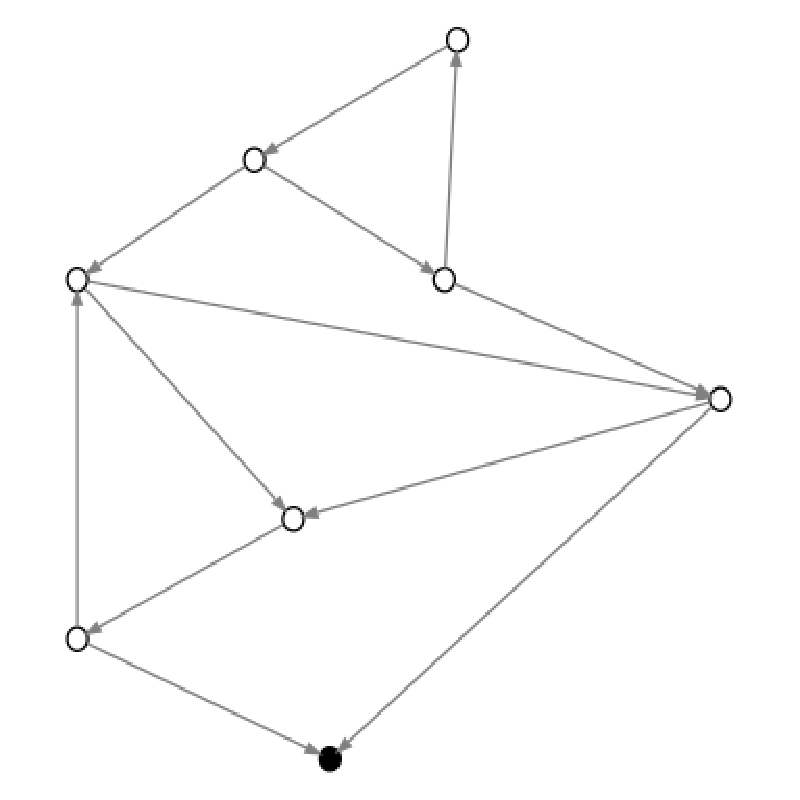
\includegraphics[scale=0.8]{images/applicationOfPrinterPipeFilterOnTarjanModel-phase-PrinterPipeFilter-level-0.eps}
  \caption{Rappresentazione di un modello SBML mediante un grafo}
  \label{fig:simple-black-and-white}
\end{figure}
La Figura \ref{fig:simple-black-and-white} riporta il risultato di
questa funzionalit\`a applicata ad un modello SBML codificato in un
grafo. 

Il commento dell'implementazione di questa funzionalit\`a viene
rimandato alla Sezione
\ref{subsection:dotInterface-package-description} dell'appendice.

\subsection{Applicare la visita in profondit\`a}
Con questa funzionalit\`a si vuole visitare in profondit\`a il grafo
in input.

Il risultato prodotto \`e una foresta di alberi \emph{DFS}, i cui
archi sono un sotto insieme dell'insieme di archi del grafo originale,
attraversati durante la computazione.

Inoltre siamo interessati ad associare, per ogni vertice, una coppia
di interi che indica il momento in cui la visita esplora un vertice e
quando l'esplorazione del vicinato di tale vertice viene
completata. Queste informazioni possono risultare molto utili in fase
di studio del grafo; abbiamo ripreso questo spunto da
\cite{Algorithms}.

Vediamo i risultati di una sua esecuzione, dopo aver composto la
funzionalit\`a descritta nella Sezione
\ref{subsection:represent-it-in-black-and-white}. La Figura
\ref{fig:before-applying-dfs-search} riporta il grafo originale di
partenza, preso da \cite{Algorithms}:
\begin{figure}
  \centering
  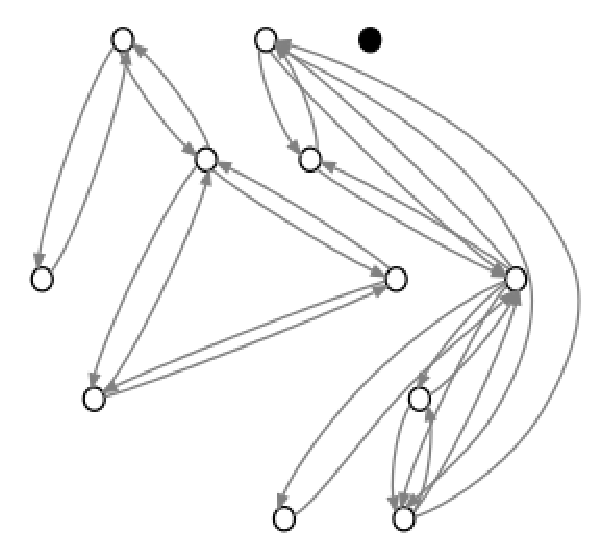
\includegraphics{images/OnePipingLevelUnitTest_Printer_DFS_PrinterPipe_Papadimitriou-phase-PrinterPipeFilter-level-0.eps}
  \caption{Grafo che si vuole visitare}
  \label{fig:before-applying-dfs-search}
\end{figure}
visitandolo in profondit\`a otteniamo la foresta di alberi \emph{DFS}
riportata in Figura \ref{fig:dfs-forest}.
\begin{figure}
  \centering
  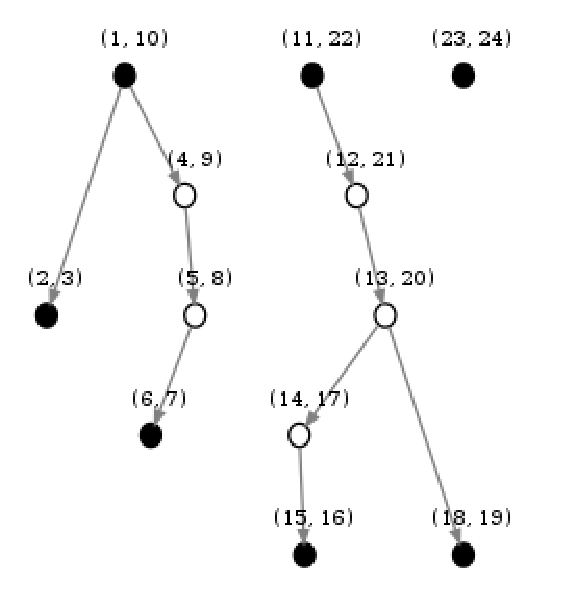
\includegraphics{images/OnePipingLevelUnitTest_Printer_DFS_PrinterPipe_Papadimitriou-phase-PrinterPipeFilter-level-2.eps}
  \caption{Risultato della visita in profondit\`a del grafo riportato
    in Figura \ref{fig:before-applying-dfs-search}}
  \label{fig:dfs-forest}
\end{figure}

Il commento dell'implementazione di questa funzionalit\`a viene
rimandato alla Sezione \ref{subsection:model-package-description}
dell'appendice.

\subsection{Applicare l'algoritmo di Tarjan}
\label{subsection:use-case-tarjan}
Con questa funzionalit\`a si vuole applicare l'algoritmo di Tarjan per
la ricerca delle componenti fortemente connesse al grafo in input.

Il risultato prodotto \`e un grafo che ha come nodi le componenti
fortemente connesse e come archi la relazione di vicinato tra le
componenti.

Inoltre siamo interessati ad associare, per ogni vertice, un intero
che indica la cardinalit\`a della componente fortemente connessa che
esso rappresenta.

Vediamo i risultati di una sua esecuzione, dopo aver composto la
funzionalit\`a descritta nella precedente Sezione
\ref{subsection:represent-it-in-black-and-white}: la Figura
\ref{fig:before-applying-tarjan} riporta il grafo originale di
partenza, preso da \cite{Algoritmica}:
\begin{figure}
  \centering
  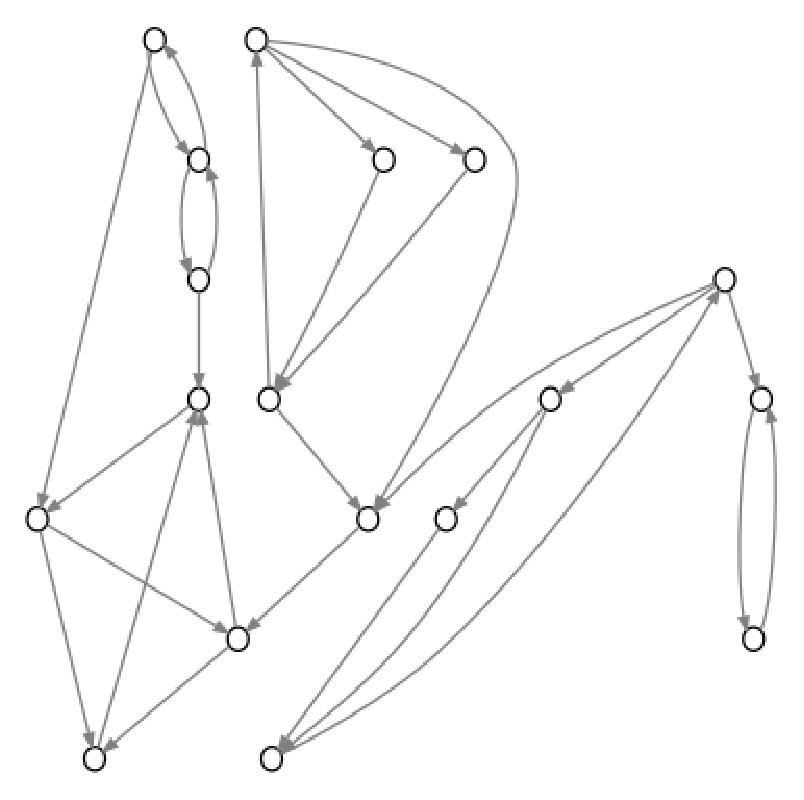
\includegraphics{images/OnePipingLevelUnitTest_Printer_DFS_PrinterPipe_Crescenzi-phase-PrinterPipeFilter-level-0.eps}
  \caption{Grafo di cui si vuole ricercare le componenti fortemente
    connesse}
  \label{fig:before-applying-tarjan}
\end{figure}
applicando l'algoritmo di Tarjan a tale grafo otteniamo la
minimizzazione riportata in Figura \ref{fig:tarjan-output}.
\begin{figure}
  \centering
  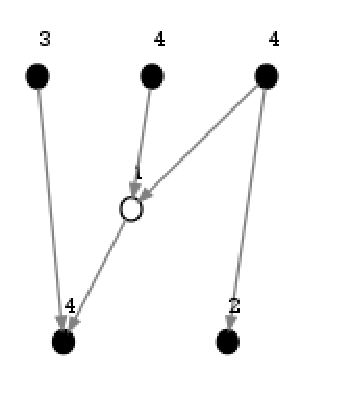
\includegraphics{images/OnePipingLevelUnitTest_Printer_DFS_PrinterPipe_Crescenzi-phase-PrinterPipeFilter-level-2.eps}
  \caption{Componenti fortemente connesse del grafo riportato in
    Figura \ref{fig:before-applying-tarjan}}
  \label{fig:tarjan-output}
\end{figure}

\subsection{Rappresentazione tabulare}
Con questa funzionalit\`a si vuole rappresentare il grafo in input in
formato testuale, usando uno schema tabellare.

Il \emph{side-effect} prodotto \`e collezionare le informazioni
richieste visitando il grafo e scriverle in un file dedicato.

Inoltre, per comodit\`a, vogliamo comporre pi\`u di una funzionalit\`a
ed avere le informazioni relative alle computazioni di ognuna,
presenti nello stesso documento.

Vediamo i risultati di una sua esecuzione, allegando un documento
prodotto:
\begin{lstlisting}
phase-PlainTextStatsPipeFilter-level-2
NOfVertices: 1
	NOfComponents:	206
	NOfEdges:	183
	NOfSources:	108
	NOfSinks:	96
	NOfWhites:	2

NOfVertices: 2
	NOfComponents:	9
	NOfEdges:	1
	NOfSources:	1
	NOfSinks:	8
	NOfWhites:	0

NOfVertices: 3
	NOfComponents:	5
	NOfEdges:	0
	NOfSources:	0
	NOfSinks:	5
	NOfWhites:	0

NOfVertices: 4
	NOfComponents:	1
	NOfEdges:	0
	NOfSources:	0
	NOfSinks:	1
	NOfWhites:	0

NOfVertices: 396
	NOfComponents:	1
	NOfEdges:	89
	NOfSources:	0
	NOfSinks:	0
	NOfWhites:	1

phase-PlainTextStatsPipeFilter-level-0
	NOfVertices:	639
	NOfEdges:	2209
	NOfSources:	108
	NOfSinks:	95
	NOfWhites:	436

\end{lstlisting}
Questo output necessita di alcune spiegazioni. Quello riportato \`e il
documento che viene generato da questa funzionalit\`a, collezionando
in un primo momento le informazioni sul grafo originale (riportate
sotto l'etichetta \emph{phase-PlainTextStatsPipeFilter-level-0}) e in
un secondo momento, dopo aver applicato l'algoritmo di Tarjan, le
informazioni sul grafo minimizzato (riportate sotto l'etichetta
\emph{phase-PlainTextStatsPipeFilter-level-2}).

Come si nota i formati delle rappresentazioni tabulari sono vicini ma
non identici. Dato il seguente blocco relativo al primo passo:
\begin{lstlisting}
phase-identifier
	NOfVertices:	v
	NOfEdges:	e
	NOfSources:	s
	NOfSinks:	d
	NOfWhites:	w
\end{lstlisting}
allora il grafo in input $G = (V, E)$, al passo
\emph{phase-identifier}, \`e tale che $|E| = e$ e $|V| = v$, di cui
$s$ vertici sono sorgenti, $d$ vertici sono pozzi e $w (= v -s -d)$
sono intermedi.

Definiamo adesso la semantica associata alle informazioni collezionate
per il secondo passo. Come si pu\`o notare, queste informazioni
ripetono uno schema, del quale \`e sufficiente dare la semantica,
quante volte \`e necessario per elencare tutti i dati raccolti. Sia
dato il \emph{template}:
\begin{lstlisting}
NOfVertices: v
	NOfComponents:	c
	NOfEdges:	e
	NOfSources:	s
	NOfSinks:	d
	NOfWhites:	w  
\end{lstlisting}
allora nel grafo minimizzato esistono $c$ componenti fortemente
connesse, ognuna delle quali raggruppa $v$ vertici. Esistono $e$ archi
uscenti in totale dalle $c$ componenti e queste sono partizionate in
$s$ componenti sorgenti, $d$ componenti pozzo e $w$ componenti
intermedie.

Come abbiamo detto ad inizio sezione, questa funzionalit\`a non
trasforma il grafo in input, anzi \`e ortogonale ad un'intera
composizione di funzionalit\`a in quanto, elencando i dati raccolti
per ogni specifico \emph{phase-identifier}, non ha dipendenze da
ognuna di esse.

Il commento dell'implementazione di questa funzionalit\`a viene
rimandato alla Sezione \ref{subsection:model-package-description}
dell'appendice.

\subsection{Ridurre la complessit\`a collassando i nodi sorgente}
Con questa funzionalit\`a si vuole eliminare tutti i vertici sorgenti
contenuti nel grafo in input, introducendo al loro posto un nuovo
vertice sorgente, tale che il suo vicinato sia uguale all'unione dei
vicinati dei vertici rimossi.

Vediamo i risultati di una sua esecuzione, applicando la
minimizzazione al grafo di input, dopo aver composto la funzionalit\`a
descritta nella precedente Sezione
\ref{subsection:represent-it-in-black-and-white}:
\begin{lstlisting}
phase-PlainTextStatsPipeFilter-level-1
	NOfVertices:	386
	NOfEdges:	1339
	NOfSources:	1
	NOfSinks:	85
	NOfWhites:	300
\end{lstlisting}
Come si vede dalle informazioni riportate, il nuovo grafo, input per
successive computazioni, ha un solo vertice sorgente.

Il commento dell'implementazione di questa funzionalit\`a viene
rimandato alla Sezione \ref{subsection:model-package-description}
dell'appendice.


\subsection{Indagare propriet\`a di una batteria di modelli}
\label{subsection:use-case-result-viewer}
Con questa funzionalit\`a si vuole rappresentare informazioni relative
ad una batteria di modelli, dei quali abbiamo calcolato le componenti
fortemente connesse, attraverso una semplice GUI utilizzando il
framework \emph{SWING}.

In realt\`a quello che ci piacerebbe costruire \`e un visualizzatore
di strutture dati, costruite appositamente per contenere le
informazioni di interesse, senza essere dipendenti dal risultato di
una computazione appena conclusa. Ovvero, vorremmo serializzare tale
struttura dati in una path del file system e poterla visualizzare
successivamente. Questo secondo noi \`e un approccio pi\`u modulare in
quanto permette di creare strutture dati e poterle scambiare,
utilizzando la maschera come semplice \emph{render}, anche se non
abbiamo generato noi stessi la serializzazione delle informazioni.

Inoltre siamo interessati a condurre la nostra indagine restringendosi
non solo ad un modello (e quindi ad un solo grafo), bens\`i vorremmo
analizzare un insieme di modelli affinch\'e sia possibile studiare in
che tipo di componente fortemente connessa ogni metabolito incontrato
appare.

\begin{figure}
  \centering
  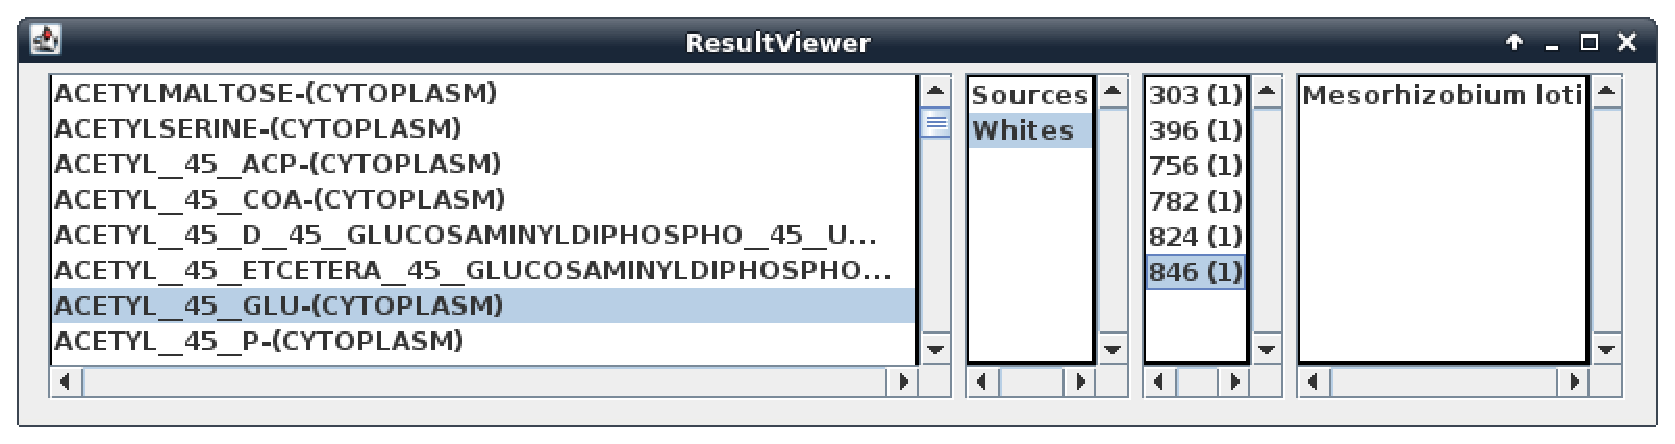
\includegraphics[scale=.5,
  angle=90]{images/ResultViewer-execution.eps}
  \caption{Visualizzatore dell'indagine relativa ad un insieme di
    modelli}
  \label{fig:result-viewer-scc}
\end{figure}
La Figura \ref{fig:result-viewer-scc} riporta uno screenshot, diamo
adesso la semantica delle informazioni rappresentate nella maschera.

Il frame contiene i seguenti componenti, che andiamo a descrivere
seguendo l'ordine da sinistra verso destra e dall'alto verso il basso:
\begin{itemize}
\item una tabella dove vengono elencati tutti i modelli che sono stati
  oggetto di indagine. Per ogni modello si associano tre coppie $(c,
  v)$ per tre colonne, ognuna rappresentante una tipologia di vertice
  (\emph{sources, whites, sinks}). Per esempio, se una coppia $c, v$
  appartiene alla riga del modello $m$ e alla colonna $whites$, allora
  significa che nel modello $m$ esistono $c$ componenti fortemente
  connesse di tipo $whites$, le quali contengono in totale $m$ vertici
  (che di conseguenza hanno pure loro il ruolo di $whites$);
\item una \emph{list-box} nella quale sono riportate delle
  informazioni relative ai metaboliti. Ogni oggetto raggruppa i
  metaboliti in base ai ruoli (ovvero in base alla tipologia di
  vertice) che hanno in tutti i modelli analizzati.

  Inoltre si calcola anche una loro frequenza in percentuale per avere
  un raffronto immediato riguardo alla predominanza dei ruoli svolti:
  si considerano tutte le possibili combinazioni dell'insieme
  ${sources, whites, sinks}$, escludendo l'insieme vuoto;
\item nella successiva \emph{list-box} vengono elencate tutte i
  metaboliti contenuti in almeno uno dei modelli oggetto
  dell'indagine. Ogni metabolito \`e codificato con una stringa
  composta dall'identificatore e, tra parantesi tonde, il nome del
  compartimento in cui risiede;
\item cliccando su un metabolito $s$, nella successiva \emph{list-box}
  vengono elencati i tipi delle componenti fortemente connesse che
  contengono il metabolito $s$;
\item cliccando su una tipologia $t$ di componente fortemente
  connessa, nella successiva \emph{list-box} vengono elencate le
  cardinalit\`a delle componenti fortemente connesse che contengono il
  metabolito $s$ e sono di tipologia $t$. Ad ogni cardinalit\`a si
  concatena un numero intero che indica la cardinalit\`a dell'insieme
  rappresentato nell'ultima \emph{list-box}, che descriveremo nel
  prossimo punto;
\item cliccando su una cardinalit\`a $c$, nell'ultima \emph{list-box}
  vengono elencati i modelli, la cui applicazione dell'algoritmo di
  Tarjan, ha prodotto un grafo in cui esiste una componente fortemente
  connessa tale che contiene il metabolito $s$, \`e di tipo $t$ ed ha
  una cardinalit\`a $c$.
\end{itemize}

Non solo le ultime quattro \emph{list-box} sono contestualmente
correlate, ma anche la tabella e la \emph{list-box} con le
informazioni per tipologia di vertice lo sono. In particolare,
selezionando nella tabella una o pi\`u righe, nella \emph{list-box}
\`e possibile avere le informazioni riguardo ai metaboliti contenuti
nei modelli selezionati. Se la selezione \`e vuota, allora le
informazioni sono relative a tutti i modelli.

Inoltre abbiamo esteso queste correlazioni anche tra il percorso
selezionato nelle ultime quattro \emph{list-box} e la tabella (e di
conseguenza alla prima \emph{list-box}). Selezionando un metabolito
dalla seconda \emph{list-box} vengono selezionati in automatico nella
tabella tutti i modelli che lo contengono e, come spiegato nel
paragrafo precedente, anche la \emph{list-box} contenente le
informazioni per tipologia di vertice verr\`a aggiornata di
conseguenza.

Se si raffina il percorso, ad esempio scegliendo la tipologia di
vertice e la cardinalit\`a nelle rispettive \emph{list-box}, viene
raffinata la selezione nella tabella dei modelli.

\subsection{Analizzare un grafo non associato ad un modello SBML}
Nelle precedenti sezioni abbiamo sempre assunto di lavorare su un
modello metabolico, ma niente ci vieta di poter utilizzare la libreria
su un grafo arbitrario che costruiamo direttamente utilizzando oggetti
del nostro modello dati.

Questo rende la libreria non strettamente legata ai concetti nel campo
della biologia e, in particolare, delle reti metaboliche, restando
invece aperta ad utilizzi nel campo della teoria dei grafi (in
realt\`a il grafo riportato in Figura \ref{fig:simple-black-and-white}
non \`e altro che il grafo utilizzato da Tarjan nel suo articolo
\cite{Tarjan}.

Il commento dell'implementazione di questa funzionalit\`a viene
rimandato alla Sezione \ref{subsection:model-package-description}
dell'appendice.



% \section{Domain model}
\section{L'architettura \emph{pipes and filters}}

In questa sezione descriveremo l'architettura che vogliamo dare al
nostro lavoro, coscienti degli obiettivi espressi nelle precedenti
sezioni e delle loro caratteristiche.

Daremo prima alcune idee prese dagli articoli che hanno introdotto
quest'architettura e, nella seconda parte della sezione, vedremo come
possiamo ``metterle a punto'' nel nostro progetto.

\subsection{Cenni teorici}
Quest'architettura \`e molto usata nella pratica e vi \`e molta
letturatura da cui poter attingere, pensiamo per\`o che tornare alle
sorgenti che per prime hanno permesso la sua diffusione sia di
notevole importanza prima di analizzare le varianti e gli studi
successivi.

I volumi da cui ho studiato sono quello del Buschmann \cite{POSA} e
alla miscellanea di Coplien e Schmidt \footnote{aggiungere qui
  riferimento bibliografico al colume PLOPD1}.

\subsubsection{Basic schema}
Nella testata che apre il pattern in \footnote{aggiungere qui
  riferimento bibliografico al volume POSA1, pag. 53} compare:
\begin{quotation}
  The \emph{Pipes and Filters} architectural pattern provides a
  structure for systems that process a stream of data. Each processing
  step is encapsulated in a filter component. Data is passed through
  pipes between adjacent filters. Recombining filters allows you to
  build families or related systems.
\end{quotation}
L'idea alla base di questo pattern \`e il principio \emph{separation
  of concerns}. Quello che si vuole fare \`e dividere tutte le
responsabilit\`a del sistema in sottotask, ognuno dei quali pu\`o
essere implementato con una componente software tale che \emph{non
  abbia dipendenze} comportamentali dalle altre componenti (non \`e
client di nessun altra, non vi \`e delega di comportamento) e che
\emph{coopera} con le altre componenti usando l'output di una
componente come input per un'altra.

\`E interessante quello che aggiungono Coplien e Schmidt, pag. 431:
\begin{quotation}
  Usually, transformation of input data is done locally and
  incrementally, so that output may begin before the input is
  completely read. This means that a filter may start to work as soon
  as its predecessor produces its first result.
\end{quotation}
Questa idea \`e molto importante se vogliamo introdurre un grado
maggiore di parallelismo nel sistema (oppure distribuire la
computazione). Nel nostro lavoro questo non \`e stato possibile, in
quanto le computazioni che abbiamo incapsulato nei nostri filtri non
permettono di produrre un output che possa ritenersi un semilavorato,
pronto per essere raffinato dal filtro successivo.

\subsubsection{Consequences about filters}
Riporto una osservazione fatta in \footnote{aggiungere qui riferimento
PLOPD1, pag. 431}:
\begin{quotation}
  To preserve the independence of the framework's components, filters
  may not share a state. The only way to put the results of different
  filters together is to organize some of them into a sequence such
  that certain filters perform further transformations on the outputs
  of others. In addition, a filter should not know the identity of the
  filters preceding or following it in the computation sequence.
\end{quotation}
Lo use-case \ref{subsection:use-case-tarjan} \`e in un certo senso
quello che Coplien identifica come \emph{certain filter that perform
  further transformations...} per lo use-case
\ref{subsection:use-case-result-viewer}, in quanto quest ultimo assume
di lavorare su un grafo che sia la minimizzazione di un altro grafo
applicando l'algoritmo di Tarjan.

Aver introdotto formalmente il concetto di filtro come astrazione \`e
stato molto vantaggioso in quanto ogni computazione, sia effettiva che
di "adattamento", pu\`o essere trattata indipendentemente e in modo
trasparente alla stregua delle altre.

\subsubsection{Consequences about pipes}
Riporto ancora da Coplien, pag.432:
\begin{quotation}
  Two principally different possibilities exist for the realization of
  pipes: pipes may simply be links between filters (such as message
  calls) or they may be separate components (such as data repositories
  or sensors). A pipe's only responsibility is to transmit data
  between filters, eventually by converting their format from the one
  produced by their sender to the one required by their receiver.
\end{quotation}
Nel nostro lavoro non abbiamo avuto bisogno della complessit\`a di
modellare veri e propri oggetti \emph{pipe}, in quanto, come vedremo
nella prossima sezione, non \`e necessario adattare il formato
dell'input per coppie diverse di filtri, che sarebbe stata
responsabilit\`a di oggetti \emph{pipe}. Abbiamo quindi scelto la
modalit\`a \emph{links between filters}.

\subsection{Reification in this work}
L'implementazione di questo pattern nella libreria ha cercato di
prendere spunto di quanto detto nella sezione precedente ma allo
stesso tempo abbiamo cercato di dare un taglio che caratterizzasse
questo progetto. 

Abbiamo introdotto la classe \emph{PipeFilter} per modellare il
concetto di \emph{filtro} e, come sua propriet\`a, un riferimento al
filtro successivo, per modellare il concetto di \emph{pipe}.

Inoltre possiamo vedere la \emph{pipeline} come una coda di filtri,
dove il primo filtro ad essere inserito nella pipeline \`e il primo ad
essere eseguito. Utilizzando la terminologia usata da Buschmann, la
nostra implementazione ricade nello scenario \emph{"a pull pipeline"},
dove la computazione viene innescata dalla richiesta di un client.

Non vi \`e bisogno di logica di conversione dell'output di un filtro
per esser trattato come input per un altro, in quanto ogni filtro
lavora con l'astrazione \emph{OurModel}, anche se avremo comportamento
diverso in base al tipo di oggetti \emph{Vertex} contenuti all'interno
dell'input.

La precedente osservazione potrebbe indurre il lettore a pensare alla
nostra architettura non tanto come una pipeline, quanto come un
sistema di decoratori \footnote{aggiungere qui riferimento
  bibliografico a DP, trovare pagina in cui si discute il
  decorator}. Questa, a nostro avviso, non \`e per niente una
conclusione errata, anzi credo che indebolire il requisito di
stabilire un'ordinamento rigido dei filtri presente nel pattern
\emph{pipeline} originale, a favore di maggior dinamicit\`a e
trasparenza sul formato di input/output, porti ad una soluzione che
sarebbe stato sufficiente implementare con un tipico schema con
decoratori.


\chapter{Implementation}
\label{chapter:implementation}
In questo capitolo daremo delle informazioni di alto livello
riguardanti l'implementazione dei concetti descritti nel capitolo
\ref{chapter:study}, descrivendo la metodologia di sviluppo
utilizzata, quali paradigmi e stili di programmazione sono alla base
delle implementazioni e un breve overview sulle funzionalit\`a
incapsulate in ogni \emph{package} della libreria.

\section{TDD}

In questa sezione descriver\`o la metodologia di sviluppo che ho
adottato per sviluppare la fase di implementazione.

\subsection{Domain modelling and big-design-up-front? No thanks!}
Ho avuto delle esperienze lavorative e in alcuni corsi affrontati
durante il mio percorso di studio, dove si prediligeva un approccio
pi\`u "classico" all'ingegnerizzazione del software. Questo approccio
era composto da una consistente fase di analisi prima di avere
feedback dallo strumento pi\`u veritiero, il codice. 

Durante questa fase di analisi si identificavano le varie entit\`a che
nello sviluppo del progetto si sarebbero tramutate in classi, si
attribuivano le responsabilit\`a in modo tale che il codice dovesse
adattarsi a quanto dettato dall'analisi (\emph{e non il
  contrario...}).

Questo approccio ritengo che sia molto rigido e che non permetta uno
sviluppo dinamico e \emph{istruttivo} come invece si mira ad avere con
tecniche \emph{agile}. Per questo motivo quello che ho cercato di
seguire \`e stata la metodologia \emph{Test-Driven Development}, che
permette un "dialogo" stretto tra le idee che si vogliono implementare
e il codice che effettivamente abbiamo scritto, avendo da quest ultimo
molti feedback che in molte situazioni hanno aiutato a chiarificare le
idee di partenza.

Ho sempre avuto molta curiosit\`a sui metodi \emph{agile} e,
soprattutto, sulla metodo \emph{Test Driven Development}. Non ho mai
avuto opportunit\`a di affrontare un progetto usando queste linee idee
e ho pensato che questo lavoro potesse essere un buon banco di prova.

Il volume su cui ho cercato di apprendere questa tecnica \`e
\footnote{aggiungere riferimento bibliografico qui al volume scritto
  per intero} \emph{Test Driven Development: By Example} scritto da
Kent Beck. In questo scritto vi sono molti esempi, scritti usando il
linguaggio di programmazione \emph{Java}, anche se le idee di avere
test automatici per assicurare la qualit\`a del codice erano gi\`a
state battute in \emph{Lisp} e, dallo stesso Beck, in
\emph{Smalltalk}.

Riporto la prima frase della prefazione:
\begin{quotation}
  \emph{Clean code that works}, in Ron Jeffries' pithy phrase, is the
  goal of Test-Driven Development. Clean code that works is a
  worthwhile goal for a whole bunch of reasons...
\end{quotation}
Non posso certo dire che le mie implementazioni soddisfino la
citazione precedente (almeno per la parte \emph{that works}), per\`o
aver guidato l'intero sviluppo tramite test \`e stata una esperienza
molto istruttiva, di cui sono soddisfatto.

Nelle prossime sezioni descrivo come i \emph{tests} sono stati di
grande aiuto durante il lavoro.

\subsection{Learning tests}
Questo tipo di test sono stati scritti soprattutto durante i primi
momenti di sviluppo, e hanno avuto l'obiettivo di
familiarizzare l'utilizzo della libreria \emph{JSBML}. 

La documentazione fornita \`e estesa e ben dettagliata, per\`o ci
sono stati degli aspetti che senza aver esercitato alcuni test non era
possibile studiarli a priori.

Per questi tests ho dedicato un package dedicato, in modo da
fattorizzare in un unico contenitore tutta la logica che ho avuto
bisogno per chiarire tutti gli aspetti necessari all'avanzamento del
mio lavoro.

In \footnote{aggiungere qui riferimento bibliografico a TDD, pag 136}
viene spiegato questo "pattern" e un aspetto che non ho potuto
sperimentare direttamente in questo sviluppo, ma che penso sia
interessante notare. Se viene rilasciata una nuova versione della
libreria \emph{JSBML} abbiamo il grande vantaggio di avere delle
asserzioni che verificano i concetti che abbiamo utilizzato come
dipendenze per il nostro lavoro. Siamo interessati che nessuna di
queste \emph{assert} sia violata dal nuovo rilascio. 

Senza questi test avremo dovuto provare il software manualmente per
controllare che il comportamento non sia cambiato. Avendoli invece,
\`e sufficiente far "correre" di nuovo tutta la batteria per
assicurare che i concetti su cui ci siamo basati non abbiano subito
modifiche.

Inoltre, scrivendo alcuni \emph{learning tests} abbiamo dedotto le
seguenti propriet\`a sui modelli SBML. I seguenti test sono stati
esercitati su una batteria di modelli biologici reali, tutti con esito
positivo:
\begin{itemize}
\item sia $r$ una reazione e siano $reactants(r), products(r)$ gli
  insiemi di \emph{reagenti} e \emph{prodotti} rispettivamente. Tali
  insiemi catturano il concetto di insieme matematico, ovvero non
  contengono oggetti duplicati;
\item $\exists r,t \in Reactions: products(t) = reactants(r)$. Questa
  propriet\`a permette di avere continuit\`a tra reazioni, ovvero un
  insiemi di \emph{prodotti} di una reazione $t$ pu\`o essere
  l'insieme di \emph{reagenti} di una reazione $r$. Questa
  propriet\`a permette di costruire dei \emph{cammini metabolici}
  composti da quante reazioni si voglia;
\item ogni metabolito deve essere contenuto in un compartimento.
\end{itemize}

\subsection{Pros}
Il maggior vantaggio che ho avuto utilizzando questa metodologia \`e
stato di poter pensare ad una funzionalit\`a vestendo due
"cappelli". Dapprima ho potuto concentrarmi sul comportamento che
desideravo, quindi poter pensare solo il sistema di messaggi che i
miei oggetti si sarebbero scambiati (e questo corrisponde alla fase
\emph{test-first}), creando un \emph{test method} per catturare
l'idea.

Quando vedevo il nuovo test fallire, ho potuto dedicarmi
all'implementazione necessaria per passare il test. 

A differenza di quanto suggerisce Beck, non ho quasi mai applicato il
pattern \emph{Fake it, ('Til you make it)} \footnote{aggiungere qui
  riferimento a TDD, pag. 151}, in modo da arrivare subito alla
\emph{green bar} e procedere poi alla rimozione dei eventuali
duplicazioni o \emph{code smell} mediante refactoring, perch\`e in
molti casi l'implementazione necessaria per superare il test non era
cosi complessa da dover procedere in \emph{baby step} (usando la
terminologia di Beck).

Forse sono stato un po' troppo prolisso sotto alcuni aspetti: le mie
batterie di test contano un totale di 191 metodi di test. Magari si
sarebbe potuto risparmiare qualcosina, per\`o quasta granularit\`a
fine penso sia stata di aiuto nella fase di superamento del test, la
maggior parte delle volte la logica da implementare non \`e stata
difficoltosa.

\subsection{Cons}
Una nota negativa che ho registrato riguarda il grado di profondit\`a
(se si vuole di precisione) che ho associato ai test pi\`u critici.

Nella parti pi\`u delicate mi sono sempre chiesto se i test scritti
era sufficienti a catturare il comportamento che effettivamente avrei
voluto. In alcuni punti ho dovuto ricorrere al debugger, ma penso che
questo sia accettabile, per aiutarmi a capire se qualche aspetto
necessit\`a di maggior copertura da parte dei metodi di test.

Parte di questi dubbi penso derivino anche della mia non esperienza
riguardo questo metodo.

Un altro punto in cui ho avuto difficolt\`a e che mi distacco da
quello che esprime Beck, riguarda lo stile con cui ho scritto le mie
asserzioni. In \footnote{aggiungere qui riferimento bibliografico a
  TDD, pag. 157}, Beck suggerisce di essere il maggior precisi
possibile nella scrittura di una \emph{assert}, riporto un esempio:
\begin{quotation}
  I've seen assertions like \emph{assertTrue(rectangle.area() !=
    0)}. You could return anything not null and satisfy this test, so
  it isn't very useful. Be specific. If the area should be 50, then
  say that it should be 50: \emph{assertEquals(50, rectangle.area())}.
\end{quotation}
Credendo nei principi espressi nella sezione
\ref{sec:objects-oriented-functional-paradigms}, quindi riducendo
l'uso di metodi accessori, ho avuto difficolt\`a a seguire i consigli
di Beck. Penso per\`o di aver recuperato usando un altra idea che
ritengo molto importante per la scrittura di solidi metodi di test: la
\emph{triangolazione} \footnote{aggiugere qui riferimento
  bibliografico a TDD, pag.153}. 

Questa idea mi ha permesso di utilizzare un approccio molto "chiuso"
per quanto riguarda l'uso di accessori, usando messaggi con lo
stile \emph{isSomethingEquals(...)}, e scrivere lo stesso metodi di
test solidi. Ad esempio:
\begin{lstlisting}
  @Test
  public void matchSpeciesCompartement() {
    Vertex v1 = VertexFactory.makeSimpleVertex();
    Vertex v2 = VertexFactory.makeSimpleVertex();
    Assert.assertNotSame(v1, v2);
    Assert.assertTrue(v1.matchCompartmentWith(v2));
    Assert.assertTrue(v2.matchCompartmentWith(v1));
    Assert.assertFalse(v1.matchSpeciesWith(v2));
    Assert.assertFalse(v2.matchSpeciesWith(v1));
  }
\end{lstlisting}
Usando questo schema, anche se il metodo \emph{matchCompartmentWith()}
invocato sull'oggetto \emph{v1} restituisse un valore fittizio solo
per superare il test, la seguente invocazione su \emph{v2} lo
contraddirrebbe, fallendo il test.


\section{Pure object-oriented and functional programming paradigms}
\label{sec:objects-oriented-functional-paradigms}

In questa sezione descriveremo le idee fondamentali e i principi che
abbiamo cercato di rispettare durante la fase di
implementazione.

Questi concetti vengono ripetuti ed usati molte volte nel codice: in
alcuni casi possono rendere la lettura del codice e lo studio pi\`u
problematico rispetto alle controparti "procedurali", ma hanno i
grandi valori aggiunti di portare maggior flessibilit\`a e
manutenibilit\`a delle astrazioni.

Ogni sottosezione ha come titolo una massima, che pu\`o sembrare un po
"stravagante" ma penso che sia un potente mezzo di comunicazione.

\subsection{Getters and setters are evil}
Riporto quello che dice Holub nel suo volume \footnote{aggiungere qui
  riferimento bibliografico a "Holub on Pattern", pag. 27}:
\begin{quotation}
  [...] it's a fundamental precept of OO systems that an object not
  expose any of its implementation details. This way, you can change
  the implementation without needing to change the code that uses the
  object. It follows that you should avoid getter and setter
  functions, which typically do nothing but provide access to
  implementation details (fields), in OO systems.
\end{quotation}

Quello che dice Holub ritengo sia il vero principio che permette ai
sistemi di essere \emph{flessibili}, nonostante non sia facile da
rispettare in tutte le situazioni. La programmazione procedurale aveva
come conseguenza l'esistenza di tante funzioni su un insieme di
argomenti, ognuna delle quali si pu\`o considerare un "piccolo
controller", capace di decidere e applicare della logica in base agli
argomenti a disposizione.

Con l'introduzione dell'astrazione \emph{object} e il mantra
\emph{everything is an object}, possiamo ridurre l'esistenza di questi
controller e dare potere decisionale sul comportamento da eseguire
agli oggetti stessi. Di conseguenza gli oggetti non sono delle
\emph{struct}ure passive, ma raggiungono maggior potenza quando quello
che modellano \`e solo comportamento.

Quindi seguendo quello che propone Holub, le informazioni devono
circolare all'interno del sistema, certo, ma se minimizziamo la
presenza di metodi accessori (termine che accomune sia metodi
\emph{get} che \emph{set}) possiamo modellare un sistema dove esistono
solo oggetti che si scambiano messaggi e non dove esistono dei
\emph{chunk} adibiti a immagazzinare informazioni, per essere usati da
oggetti "privilegiati".

Nel mio codice un esempio di quanto affermato sopra \`e il contratto
\emph{Vertex}, il quale, come analizzato nei capitoli precedenti, ha
come informazioni salienti: identificatore, nome, compartimento e
vicinato. Quello che il contratto richiede ad un oggetto per essere
considerato un \emph{Vertex} (detto cos\`i sembra molto lo stile
\emph{duck typing} dei linguaggi dinamici, in Java \`e pi\`u corretto
dire che la classe deve implentare tutte le caratteristiche richieste
dal contratto affinche sulle sue istanze si possano invocare tali
metodi) non \`e \emph{getIdentifier()} o \emph{getNeighborhood()},
bensi:
\begin{lstlisting}
  boolean isYourNeighborhoodEquals(Set<Vertex> products);
  boolean isYourNeighborhoodEmpty();
  boolean isYourSpeciesId(String speciesId);
  boolean isYourCompartmentId(String compartmentId);
  boolean isYourSpeciesName(String species_name);
\end{lstlisting}
quello che si st\`a chiedendo non \`e tanto una azione passiva, ma un
controllo attivo a cui solo il destinatario pu\`o rispondere in modo
univoco.

Si pu\`o andare oltre, in quanto il tipo di ritorno \emph{boolean},
pu\`o invogliare a scrivere logica condizionale (altro \emph{smell}
che ritengo sia da minimizzare), nella prossima sezione vedremo
come si potrebbe far meglio.

\subsection{Don't ask, tell!}

Riporto ancora da Holub, marcato in grassetto nel suo volume
\footnote{sempre riferimento a Holub on Patterns, pag 30}:
\begin{quotation}
  Don't ask for the information that you need to do some work; ask the
  object that has the information to do the work for you.
\end{quotation}
Penso che linguaggi come Smalltalk, Ruby, Lisp incapsulino questo
principio e il linguaggio stesso sia pi\`u ricco per trattare
\emph{everything an object}. Tornando alla promessa fatta alla fine
della sezione precedente, supponiamo di voler eseguire una determinata
logica se il vicinato di un vertice \`e vuoto. In Java dovremo
scrivere:
\begin{lstlisting}
  if(vertex.isYourNeighborhoodEmpty()){
    // do some ugly logic...
  }
\end{lstlisting}
In Smalltalk invece:
\begin{lstlisting}
  vertex isYourNeighborhoodEmpty ifTrue: anUglyBlock
\end{lstlisting}
La differenza \`e che nella versione Java la conoscenza sul vicinato
adesso \`e in due punti, sia nella classe concreta di cui
\emph{vertex} \`e una istanza, sia nella classe a cui appartiene il
blocco di codice riportato.

Nella versione Smalltalk invece la conoscenza sul vicinato \`e
incapsulata all'interno dell'oggetto \emph{vertex} e in nessun altro
punto, in quanto il codice client riportato, passa al metodo
\emph{ifTrue} un \emph{block} da eseguire a discrezione dell'oggetto
\emph{vertex} (\emph{don't ask, tell!}) se il suo vicinato \`e vuoto.

Quanto detto nell'ultima frase porta naturalmente ad un paradigma
chiave del paradigma funzionale, che descriviamo nella prossima
sezione.

\subsection{Functions (or better, behaviours) as values}



Nella prossime sezioni faremo una breve panoramica sui package che
contengono le implementazioni.

\section{Packages' descriptions}
\label{section:packages-descriptions}

Nelle prossime sezioni descriveremo gli oggetti implementati nei
\emph{packages} java. Ogni package verr\`a descritto in una sezione
dedicata, dandone i concetti principali, alcuni diagrammi usando la
notazione \emph{UML} e alcuni dettagli implementativi di interesse ed
eventuali design patterns and coding idioms che hanno aiutato
nell'implementazione.

\subsection{Pacchetto dotInterface}
\label{subsection:dotInterface-package-description}
Questo pacchetto incapsula tutte quelle astrazioni necessarie alla
creazione di un documento compilabile con i motori messi a
disposizione dalla libreria \emph{graphviz}.

\subsubsection*{Funzionalit\`a implementate}

Le funzionalit\`a fornite da questo pacchetto sono le seguenti:
\begin{itemize}
\item definire i contratti fondamentali che codificano le
  responsabilit\`a affinch\`e un oggetto sia esportabile in formato
  dot e, in modo duale, sia capace di esportare in formato dot un
  altro oggetto. Questi due contratti sono le astrazioni pi\`u
  importanti di tutto il pacchetto e sono dipendenze delle classi
  \emph{Vertex} e \emph{OurModel};
\item incapsulare in un'unica classe tutte quelle funzionalit\`a e
  caratteristiche utilizzate durante la generazione dell'output,
  alcune di esse dipendenti dal sistema operativo che ospita la
  \emph{Java Virtual Machine}, ad esempio: il separatore utilizzato
  nei percorsi di file e directory nel file system, posizioni degli
  output della libreria e delle cartelle dove trovare i modelli di
  input;
\item fornire un wrapper per oggetti di tipo \emph{Writer}, per
  concatenare alla rappresentazione testuale dell'oggetto il carattere
  `;', i due caratteri di \emph{carriege return} e \emph{new line} per
  appendere il prossimo contenuto su una nuova linea, agevolando la
  scrittura di documenti dot.
\end{itemize}

\subsubsection*{Classi}
Procediamo con ordine nel descrivere le principali classi:

\begin{paragraph}{DotExporter}
  Il contratto \emph{DotExporter} definisce quali sono i messaggi che
  un esportatore deve essere in grado di comprendere per costruire
  documenti in formato dot, lavorando su un grafo codificato con le
  astrazioni di \emph{Vertex} e \emph{OurModel}.

  I messaggi definiti in \emph{DotExporter} riguardano le componenti
  basilari di un grafo che si possono rappresentare graficamente: il
  vertice (con eventuale etichetta esterna al nodo) e l'arco (di cui
  non \`e stato necessario introdurre un'etichetta). Riporto il codice
  per maggior chiarezza:
  \begin{lstlisting}
public interface DotExporter extends DotDocumentPartHandler {
  DotExporter buildVertexDefinition(Vertex vertex);
  DotExporter collectCompleteContent(Writer outputPlugObject);
  DotExporter buildEdgeDefinition(Vertex source, Vertex neighbour);
  DotExporter buildVertexLabelOutsideBoxDefinition(Vertex vertex);
}

public interface DotExportable {
  void acceptExporter(DotExporter exporter);
}

  \end{lstlisting}
  Per non accoppiare in modo forte la modalit\`a di salvataggio
  dell'output nei messaggi dell'interfaccia, ne viene esposto uno che
  ha come argomento un oggetto di tipo \emph{Writer}, appartenente alla
  libreria di \emph{io} fornita in \emph{openjdk}.

  Questo non limita l'insieme di destinazioni dell'output, bens\`i
  lascia aperte molte scelte ed eventuali client del contratto
  \emph{DotExporter} potranno utilizzare i propri oggetti come
  destinazione dell'output, potendoli usare per computazioni
  successive. Nelle nostre implementazioni abbiamo usato quasi sempre
  oggetti di tipo \emph{FileWriter} come destinazioni concrete.
\end{paragraph}

\begin{paragraph}{DotExportable}
  Questo contratto permette di definire quali responsabilit\`a devono
  essere implementate affinch\`e un oggetto sia esportabile in formato
  dot.

  Non \`e un'interfaccia molto ricca, ma il solo messaggio
  \emph{acceptExporter} \`e sufficiente per catturare la nostra
  idea. Questa struttura si avvicina molto a quella che viene esposta
  nel pattern \emph{Visitor} in \cite{SmalltalkCompanion98}, anche se
  la nostra implementazione non la ricalca fedelmente: il taglio che
  abbiamo voluto dare alla coppia \emph{DotExporter} e
  \emph{DotExportable} usa lo stesso il \emph{double dispatch}, con la
  differenza di non esporre nel contratto \emph{DotExporter} i metodi
  relativi alle classi concrete di \emph{Vertex}, avendo un solo
  messaggio \emph{buildVertexDefinition} come sopra riportato.
\end{paragraph}






\subsection{JSBMLInterface package}

In questa sezione descriveremo il package \textbf{JSBMLInterface}.

Questo package contiene le implementazioni dei concetti che riguardano
l'interfacciamento con il modello SBML e in particolare con la
libreria JSBML (vedi \cite{JSbmlDistribution}). 

\subsubsection*{Supplied Abstractions}

Le astrazioni fornite da questo package sono le seguenti:
\begin{itemize}
\item astrarre dalla libreria JSBML e dal suo modello dati. In questo
  modo l'unico contesto del progetto dipendente dalla libreria JSBML
  \`e confinato a questo singolo package. Questo permette agli altri
  package di non essere a conoscenza della specifica "sorgente" che
  fornisce il modello, in quanto se si vorr\`a sostituire libreria di
  interfacciamento con modelli SBML, sar\`a necessario apportare le
  modifiche solo in questo package, lasciando tutto il restante codice
  del progetto inalterato.
\item interpretare il modello fornito dalla libreria JSBML, costruire
  gli elementi fondamentali del nostro modello dati e renderlo
  disponibile per iniziare successive computazioni.
\end{itemize}

\subsubsection*{Class diagram}

Riporto una versione semplificata del diagramma delle classi di questo
pacchetto, disegnando solo quelle classi di interesse per la
trattazione.
\begin{figure}
  \centering
  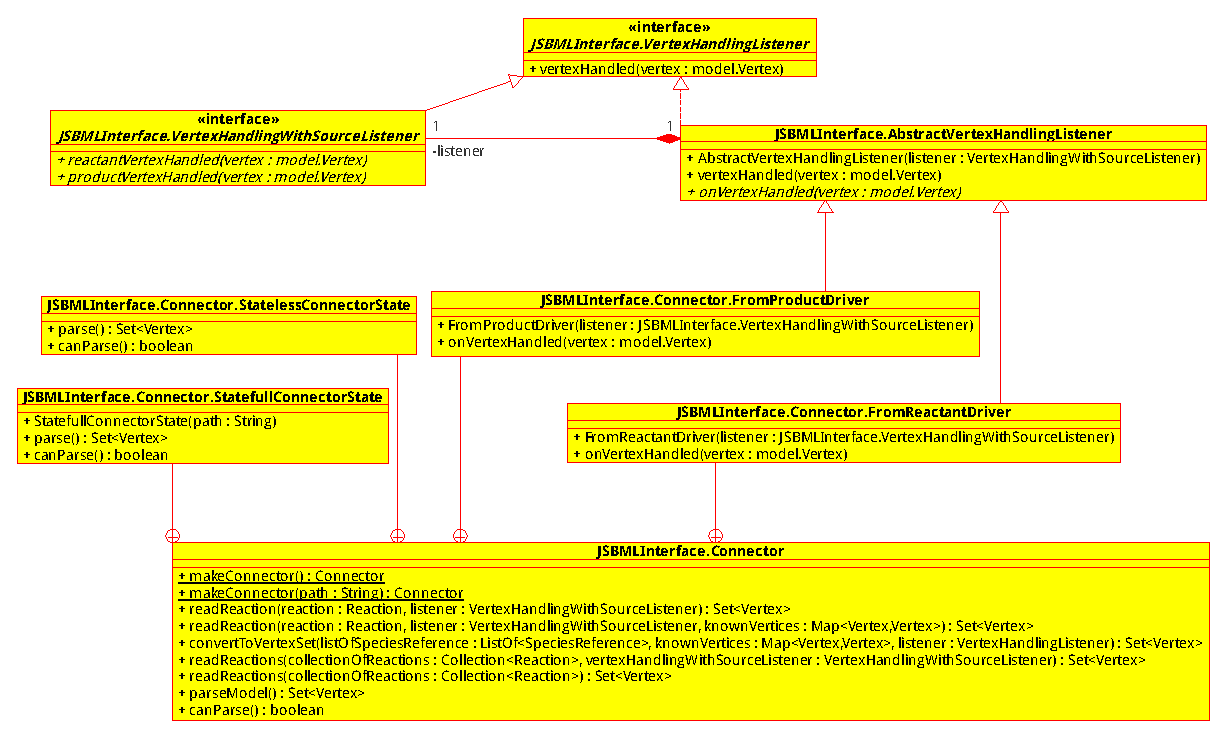
\includegraphics[angle=90]{packages/JSBMLInterface-class-diagram.eps}
  \caption{JBSMLInterface package's classes}
  \label{fig:JSBMLInterface-ClassDiagram}
\end{figure}

In questo package la classe principale e che merita qualche
spiegazione \`e \emph{Connector}.

Questa classe incapsula la responsabilit\`a di delegare alla libreria
JSBML la lettura di un modello SBML e successivamente interpretare il
risultato di tale lettura in modo da costruire un nostro modello dati
interno, input di successive computazioni.

La parte di interpretazione del modello letto dalla libreria JSBML \`e
quella pi\`u interessante, in quanto permette di elaborare e
selezionare solo quelle informazioni del modello SBML che
effettivamente sono necessarie al nostro lavoro, come descritto nella
sezione "\nameref{sec:necessaryRealObjectsModeledInSBML}". 

Questo procedimento \`e implementato principalmente nel metodo
\emph{readReactions}, il quale permette di costruire un insieme di
vertici che verranno usati per costruire il nostro modello di dominio,
a partire da una collezione di reazioni, risultato della lettura della
libreria SBML. Inoltre, come spiegher\`o nella prossima sezione, \`e
possibile passare come argomento un \emph{listener} da notificare ogni
qualvolta si costruisce un nuovo vertice per il modello da costruire.

Quello che viene fatto \`e di scandire ogni reazione e, per ognuna, si
creano tanti vertici tanti sono gli oggetti appartenenti agli insiemi
\emph{reactants} e \emph{products}, prestando attenzione a non
costruire nuovi vertici per species gi\`a analizzate.
\subsection{Pacchetto Model}
\label{subsection:model-package-description}
Questo pacchetto contiene le implementazioni dei concetti che riguardano
le pi\`u importanti e ricche astrazioni del progetto.

\subsubsection*{Funzionalit\`a implementate}
\label{subsection:model-supplied-abstractions}
Le funzionalit\`a fornite da questo pacchetto sono le seguenti:
\begin{itemize}
\label{itemize:model-supplied-abstraction}
\item definire l'astrazione di vertice e delle sue specializzazioni,
  necessarie per implementare gli altri moduli del
  progetto. Quest'astrazione pu\`o essere modellata a livello teorico
  con un \emph{abstract data type}, in quanto non vogliamo che i
  client siano a conoscenza delle specifiche realizzazioni (come
  invece lo sarebbe se fosse stato un \emph{algebraic data type}),
  vogliamo invece usare un approccio trasparente per mantenere
  flessibile il sistema. Le specializzazioni del concetto di vertice
  che abbiamo implementato sono quelle di vertice semplice, di vertice
  da usare nella visita in profondit\`a e negli algoritmi per la
  ricerca delle componenti fortemente connesse. Per la creazione di
  questi oggetti si utilizzano degli oggetti \emph{factory} (vedi
  relativo pattern in \cite{SmalltalkCompanion98});
\item implementare l'astrazione di grafo, arricchendola con
  comportamenti per poterne modificare la struttura ed eseguire delle
  computazioni su di esso: \`e possibile usare due idee prese dal
  paradigma funzionale per agire sui vertici del grafo ed \`e fornita
  una implementazione della visita in profondit\`a che espone i punti
  di estensione come esposto nella Sezione
  \ref{subsection:dfs-extension-point};
\item interfacciare le astrazioni di vertice e grafo con gli oggetti
  definiti nel pacchetto \emph{DotInterface}, per darne una
  rappresentazione grafica che riporti le idee definite nell'articolo
  \cite{tellingStories}.
\end{itemize}

\subsubsection*{Classi}
Procediamo con ordine nel descrivere le idee principali catturate in
ogni contratto:

\begin{paragraph}{Vertex}
  L'interfaccia \emph{Vertex} \`e l'astrazione principale dell'intera
  libreria.  Tramite \emph{Vertex} possiamo richiedere ad un valido
  implementatore di gestire le informazioni sul vicinato di un
  vertice, dando la possibilit\`a sia di aggiungere vicini che
  predecessori (quindi modelliamo sia una lista di adiacenza, sia una
  lista di incidenza). Questo ci permette di avere un costo
  nell'ordine $O(m + n)$ dove $m$ \`e il numero totali di archi ed $n$
  \`e il numero di nodi presenti nel grafo codificato nel nostro
  modello. Inoltre, per poter collassare le sorgenti in una unica, \`e
  possibile richiedere la ``rottura'' della relazione di vicinato per
  poter successivamente cancellare il vertice dal grafo.

  \emph{Vertex} permette di richiedere informazioni sulle
  caratteristiche del vertice, ad esempio se un vertice \`e sorgente o
  pozzo, qual \`e il suo vicinato, quali sono le informazioni che lo
  distinguono (riferite alla metabolito e al compartimento recuperate
  dal modello SBML di origine).

  Tramite questo contratto possiamo interfacciare le implementazioni
  definite nel pacchetto \emph{dotInterface}, richiedendo di accettare
  un esportatore per costruire un documento in formato \emph{dot}.

  \`E possibile richiedere anche delle informazioni di carattere
  testuale rappresentandole in una tabella, dalle quali si pu\`o
  capire meglio la struttura del grafo.

  Una propriet\`a che questo contratto richiede \`e quella di
  riscrivere i metodi \emph{equals} e \emph{hashCode} in modo che
  tutti gli oggetti implementatori di questa interfaccia possano
  essere trattati come \emph{value objects}, non distinguendoli per
  riferimento in memoria (implementazione di default del metodo
  \emph{equals} fornito da \emph{openjdk}), bens\`i per le
  informazioni che questi incapsulano (e quindi poter usare
  \emph{late-binding} ed avere comportamento polimorfo in base
  all'oggetto che riceve i suddetti messaggi). Abbiamo effettuato
  questa scelta in modo da poter creare implementatori di
  \emph{Vertex} all'occorrenza con le stesse caratteristiche, senza
  dover gestire una struttura dati per la memorizzazione e la ricerca
  dell'unico oggetto creato.

  Come ultima propriet\`a, questo contratto impone una relazione
  d'ordine totale sull'insieme degli implementatori, in modo da
  rendere gli algoritmi deterministici nel momento di selezione dei
  vertici.
\end{paragraph}

\begin{paragraph}{OurModel}
  La classe concreta \emph{OurModel} implementa l'astrazione grafo da
  utilizzare come modello di dominio per le computazioni descritte nel
  Capitolo \ref{chapter:study}.

  La prima responsabilit\`a di \emph{OurModel} \`e costruire il
  modello in diverse modalit\`a: a partire da un insieme di vertici
  gi\`a costruiti (quindi con le relazioni di vicinato gi\`a fissate)
  oppure a partire da un modello SBML esistente in una path del file
  system.

  La seconda \`e templetizzare l'algoritmo della visita in
  profondit\`a, introducendo dei punti di estensione sui quali \`e
  possibile ``personalizzare'' il comportamento della visita ed
  implementare delle varianti. Quelle che abbiamo implementato in
  questo lavoro sono quelle definite nel Capitolo
  \ref{chapter:theoretical-background}, ma questo non limita un
  utilizzatore della libreria di definire il proprio comportamento e
  di usare l'implementazione della visita per algoritmi che non
  abbiamo trattato.

\end{paragraph}

\begin{paragraph}{Implementazioni di Vertex}
  Abbiamo molti comportamenti diversi che vogliamo poter utilizzare
  come istanze dell'astrazione definita dal contratto
  \emph{Vertex}. Il vantaggio di aver implementato il codice
  riferendosi sempre al contratto e non alle singole caratterizzazioni
  \`e di essere trasparente e poter interscambiare i comportamenti
  specifici, lasciando immutato il codice che implementa i vari
  algoritmi.

  Vediamo quali sono gli implementatori del contratto \emph{Vertex},
  descrivendoli brevemente.

  La prima implementazione introdotta \`e stata \emph{SimpleVertex},
  che cattura il comportamento di un vertice ``normale'', ovvero
  l'implementazione pi\`u semplice possibile del contratto. Anche se
  pu\`o sembrare scontata, \`e il mattone utilizzato pi\`u o meno
  indirettamente dalle implementazioni pi\`u complesse: queste sono
  dei \emph{wrapper} che delegano la maggior parte del comportamento a
  questa implementazione base, ridefinendo solo i metodi per i tratti
  che le distinguono.

  La seconda implementazione introdotta \`e stata
  \emph{DfsWrapperVertex}, che associa l'analogo di un ``timestamp''
  nei momenti in cui la visita in profondit\`a raggiunge un vertice e
  in cui lo abbandona. 

  La terza implementazione introdotta \`e stata
  \emph{ConnectedComponentWrapperVertex}, in coppia con
  \emph{TarjanWrapperVertex}. Queste implementano, in modo puramente
  orientato agli oggetti, l'algoritmo per la ricerca delle componenti
  fortemente connesse. In particolare
  \emph{ConnectedComponentWrapperVertex} rappresenta una componente
  fortemente connessa e mantiene l'insieme dei vertici del grafo di
  origine di cui \`e composta, mentre \emph{TarjanWrapperVertex}
  cattura la responsabilit\`a di mantenere la relazione di vicinato
  tra le componenti fortemente connesse. Inoltre abbiamo introdotto
  l'astrazione \emph{ConnectedComponentInfoRecorder} per poter
  sviluppare un semplice programma per la visualizzazione di semplici
  statistiche come descritto nel Capitolo \ref{chapter:study}.

  L'implementazione \emph{VertexWithLabelWrapperVertex}, ortogonale
  alle precedenti, riporta un'etichetta sopra alla rappresentazione di
  un vertice nella generazione dell'output grafico. Questo
  comportamento \`e possibile utilizzarlo in modo trasparente e
  permette di fattorizzare il codice che cattura la decorazione da
  quello che cattura le particolari implementazioni del contratto
  \emph{Vertex}.

  Tutte le precedenti implementazioni sono nascoste ai client del
  contratto \emph{Vertex}, utilizzando \emph{VertexFactory} come unico
  mezzo per poterle costruire, esponendo un metodo statico per ogni
  implementazione che abbiamo descritto.
\end{paragraph}


\section{Piping package}

In questa sezione descriveremo il package \textbf{piping}.

Questo package contiene le implementazioni che permettono di
assemblare una \emph{pipeline}, attraverso la composizione di un
numero quanto si voglia di filtri. Descriveremo i filtri che abbiamo
implementato e come \`e possibile crearne di nuovi.

\subsection{Supplied Abstractions}

Le astrazioni fornite da questo package sono le seguenti:
\begin{itemize}
\item fornire un \emph{template} di filtro, componente atomica per la
  composizione di una \emph{pipeline}. Questo template implementa
  tutto il comportamento necessario affinch\`e possa essere combinato,
  lasciando all'implementatore il compito di codificare la logica che
  caratterizza il filtro che stiamo modellando.
\item fornire un insieme di filtri gi\`a implementati necessari alla
  realizzazione dei requisiti nella sezione
  \ref{section:use-cases}. Questi filtri permettono di generare la
  rappresentazione grafica e testuale di un grafo, di applicare una
  ricerca \emph{DFS}, di applicare l'algoritmo di Tarjan e trasformare
  un grafo collassando le sue sorgenti in una unica.
\item facilitare la creazione dei precedenti filtri attraverso una
  \emph{factory}, in modo da disaccoppiare il codice client dei filtri
  dalle classi specifiche. A differenza di quanto implementato per i
  realizzatori del contratto \emph{Vertex} (vedi
  \ref{subsection:model-supplied-abstractions}), non si vuole
  nascondere le classi che implementano le varie caratterizzazioni di
  filtro, quindi \`e possibile sia utilizzare la factory sia creare i
  filtri utilizzando i rispettivi costruttori.
\item catturare ed esporre il concetto di \emph{listener}, mediante il
  quale \`e possibile essere notificati tramite degli eventi durante
  la computazione. Questi eventi sono modellati tramite messaggi
  definiti in un contratto dedicato e possono essere inviati sia dal
  template che modella il filtro, sia dalla logica che caratterizza il
  comportamento che differienzia un filtro da un altro. Attraverso un
  listener \`e possibile assemblare la propria pipeline ed eseguire
  non solo le trasformazioni che questa produce, ma anche della logica
  quando determinati eventi accadono. Questo \`e uno strumento molto
  potente in quanto permette di essere ortogonali alla pipeline e aver
  un maggior grado di controllo sull'intera computazione.
\end{itemize}

\subsection{Class diagram}
Il diagramma rappresentato in figura \ref{fig:piping-package-classes}
rappresenta i concetti implementati in questo package. Procediamo con
ordine nel descrivere le idee principali catturate da ogni classe:

\begin{figure}
  \centering
  % 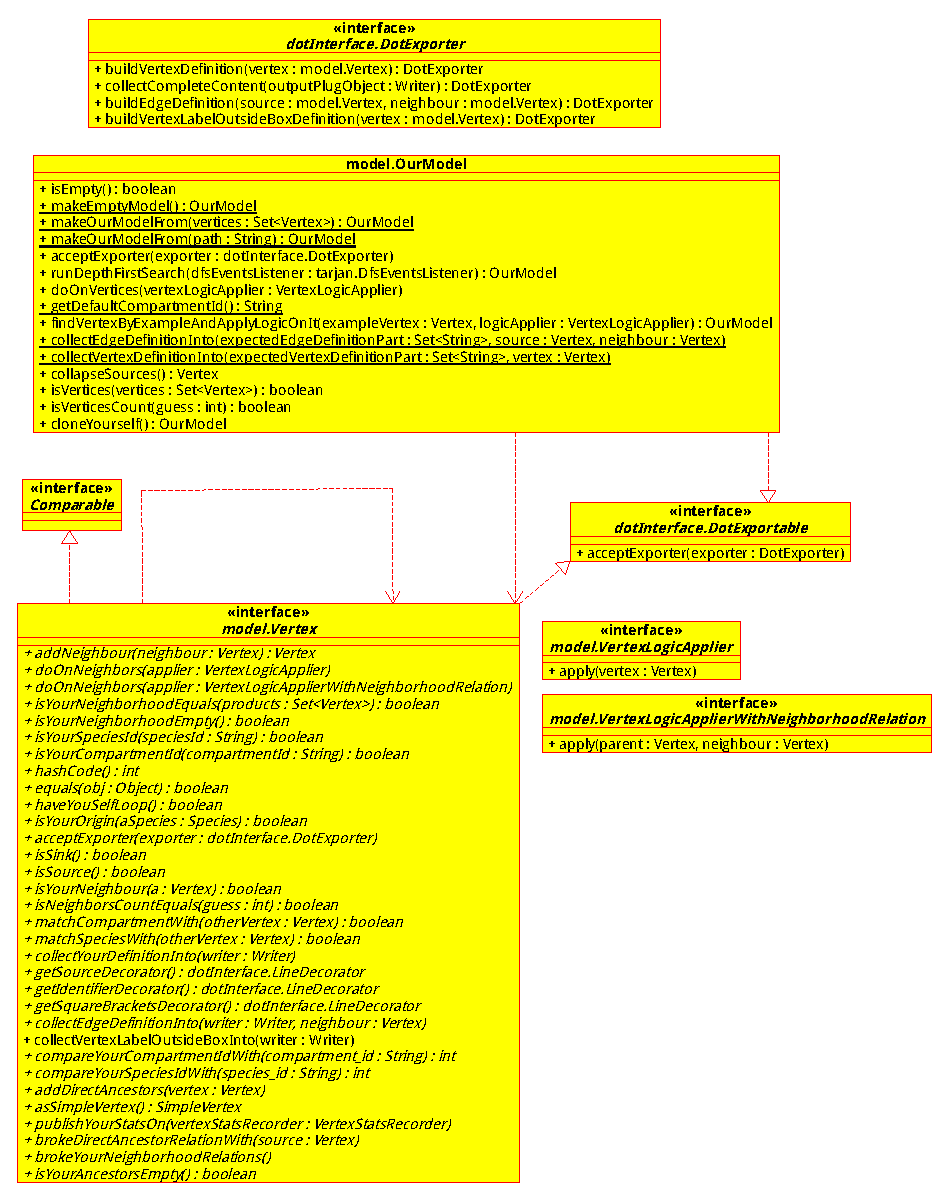
\includegraphics{packages/vertex-interface-class-diagram.eps} 
  \caption{Piping package's classes}
  \label{fig:piping-package-classes}
\end{figure}

\begin{paragraph}{PipeFilter}
  Abbiamo cercato di formalizzare in modo preciso la pi\`u piccola
  unit\`a atomica capace di eseguire una computazione all'interno di
  una sequenza pi\`u grande. Questo ci ha portato alla definizione
  della classe astratta \emph{PipeFilter}. Aver introdotto questa
  classe ci ha permesso di rendere il codice molto flessibile e
  trasparente, nonch\`e molto pi\`u facile da implementare.

  Questa classe, come abbiamo detto nei paragrafi precedenti, in
  realt\`a rappresenta solo un \emph{template} del concetto di filtro
  e non di un filtro che esegue una trasformazione sull'istanza di
  input. Le sue responsabilit\`a sono di poter assemblare una sequenza
  di filtri, utilizzando l'idea alla base della costruzione di una
  lista concatenata, ed eseguire la computazione, eventualmente
  propagando la richiesta di esecuzione a tutti i filtri che si sono
  assemblati.

  Quanto detto nel precedente paragrafo \`e stato molto semplice da
  implementare avendo data a \emph{PipeFilter} una struttura
  ricorsiva: per costruire una pipeline con due filtri \`e sufficiente
  costruirli, dare la relazione di precedenza che identifica la
  pipeline, e sul filtro pi\`u esterno invocare la richiesta di
  esecuzione. Il primo filtro che riceve tale richiesta, controlla se
  il filtro che lo precede \`e istanziato: se lo \`e allora si delega
  la richiesta di esecuzione, altrimenti, o successivamente la
  terminazione dell'esecuzione di tutti gli eventuali filtri
  precedenti, si esegue la trasformazione che caratterizza il filtro
  corrente che ha ricevuto per primo la richiesta. Inoltre, data la
  natura ricorsiva di \emph{PipeFilter}, \`e possibile comporre una
  pipeline i cui filtri sono a loro volta pipeline, oppure un mix di
  pipeline e filtri.

  L'esecuzione di una pipeline riceve come istanza di input un grafo
  codificato da un oggetto di tipo \emph{OurModel}, ed eventualmente
  un listener, questa istanza viene propagata al filtro che non ha
  predecessori. Quest ultimo esegue la sua trasformazione e ritorna un
  nuovo grafo, che diventer\`a instanza di input del suo
  successore. Si applica questa di regola di esecuzione fino a che il
  filtro pi\`u esterno della pipeline, ovvero quello che per primo ha
  ricevuto la richiesta di esecuzione, ricever\`a a sua volta una
  instanza di input, eseguir\`a la computazione e restituir\`a il
  grafo finale.

\end{paragraph}

\begin{paragraph}{Concrete \emph{PipeFilter}s}
  Come abbiamo detto, \emph{PipeFilter} rappresenta solo un
  \emph{template}: il comportamento che vogliamo dare ad ogni filtro
  deve essere codificato in una classe concreta che "completa" tale
  template. In realt\`a non \`e molto il lavoro che si lascia da
  scrivere. Per completare il template \`e sufficiente
  l'implementazione di un metodo astratto, che ha come parametri il
  grafo di input e deve ritornare una grafo utilizzato come input per
  il filtro successivo.

  Tutti i filtri che abbiamo implementato in questa libreria
  compongono il comportamento esposto da altri oggetti, fornendo nella
  maggior parte dei casi le implementazioni di \emph{hook
    methods}\footnote{aggiungere qui riferimento bibliografico al
    volume del Pree}, per ottenere la caratterizzazione desiderata.

  Il primo filtro concreto che abbiamo introdotto \`e stato
  \emph{PrinterPipeFilter}, il quale produce una rappresentazione
  grafica, producendo un documento compilabile con il programma
  \emph{dot}\footnote{aggiungere qui riferimento bibliografico alla
    libreria graphviz}. Questo filtro non apporta nessuna
  trasformazione al grafo di input e lo restituisce cosi come lo ha
  ricevuto. Per adempiere alla sua responsabilit\`a, questo filtro
  costruisce un esportatore (come descritto in \footnote{aggiungere
    qui il riferimento alla sezione del package dotInterface, ancora
    non l'ho descritto}) per visitare il grafo e collezionare tutte le
  informazioni necessarie per costruire il documento \emph{dot}.

  Il secondo filtro concreto che abbiamo introdotto \`e stato
  \emph{DfsPipeFilter}, il quale esegue una visita \emph{DFS} sul
  grafo di input e ritorna un grafo contenente solo il sottoinsieme di
  archi visitati. Concatenando come successore un filtro di tipo
  \emph{PrinterPipeFilter} sar\`a possibile visualizzare l'albero
  \emph{DFS} che rappresenta la visita eseguita.

  Il terzo filtro concreto che abbiamo introdotto \`e stato
  \emph{TarjanPipeFilter}, il quale applica l'algoritmo di Tarjan per
  la ricerca delle componenti fortemente connesse sul grafo di
  ingresso e restituisce un nuovo \emph{dag} composto dalle componenti
  identificate. \`E importante sottolineare la potenza di aver
  strutturato il codice nel modo pi\`u generico possibile, ovvero il
  grafo prodotto da questo filtro non ha come vertici dei semplici
  \emph{SimpleVertex}, bensi degli oggetti che caratterizzano le
  componenti fortemente connesse. In questo modo possiamo continuare
  ad inviare gli stessi messaggi, ad esempio componendo ancora un
  filtro \emph{PrinterPipeFilter}, ma ottenere una rappresentazione
  diversa rispetto a quella che si otterebbe dato un grafo "semplice".

  Il quarto filtro concreto che abbiamo introdotto \`e stato
  \emph{SourcesCollapserPipeFilter}, il quale permette di collassare
  tutte le sorgenti ed introdurne una nuova ed unica. Il nuovo grafo
  viene restituito per eventuali computazioni successive.

  Gli ultimi filtri concreti che abbiamo introdotto sono stati
  \emph{PlainTextStatsPipeFilter} e
  \emph{ConnectedComponentInfoPipeFilter}. Questi hanno la
  responsabilit\`a di produrre una rappresentazione testuale del grafo
  in input, producendo il primo un output tabellare, il secondo una
  serializzazione di una struttura dati che mantiene delle
  informazioni sulle componenti fortemente connesse, consultabili
  utilizzando il relativo programmetto \emph{ResultViewer}.

\end{paragraph}

\begin{paragraph}{PipeFilterComputationListener}
  Il concetto di listener \`e molto simile a quello di \emph{Observer}
  come descritto in \footnote{aggiungere qui riferimento bibliografico
    a Design Patterns}, anche se nella nostra implementazione non
  dobbiamo notificare di un cambiamento, bensi notificare che \`e
  accaduto un determinato evento. Questi eventi sono modellati come
  messaggi nell'interfaccia \emph{PipeFilterComputationListener} e per
  adesso siamo interessati alla notifica dell'inizio e della fine
  della computazione di ogni filtro.

  L'utilit\`a dei listener risiede nella possibilit\`a di ricevere
  degli argomenti inviati dal mittente della notifica ed essere
  elaborati per implementare le funzionalit\`a desiderate. Questi
  argomenti aggiuntivi possono essere relativi non solo ad uno
  specifico filtro, bensi ad un insieme di filtri, in quanto per tutta
  la durata della pipeline si usa lo stesso listener.Un esempio \`e
  \emph{PlainTextInfoComputationListener}, il quale colleziona in una
  mappa, per ogni filtro, delle informazioni che verranno utilizzate
  successivamente per produrre una rappresentazione testuale del
  grafo. Queste informazioni vengono raccolte in un oggetto dapprima
  nell'esecuzione di un filtro \emph{PlainTextStatsPipeFilter}, quando
  questo termina il suo compito, invia un messaggio al listener che la
  computazione \`e terminata, allegando come argomento l'oggetto con
  le informazioni. Questo ci ha permesso di applicare trasformazioni e
  trattare i risultati di queste in modo collettivo, senza doverle
  comporre a computazione terminata.


\end{paragraph}


\subsection{Pacchetto Tarjan}
\label{subsection:tarjan-package-description}
Questo pacchetto non contiene molte astrazioni limitandosi a definire un
contratto fondamentale per implementare la visita \emph{DFS} e
l'algoritmo per la ricerca di componenti fortemente connesse.

\subsubsection*{Funzionalit\`a implementate}
Le funzionalit\`a fornite da questo pacchetto sono le seguenti:
\begin{itemize}
\item definire il contratto nel quale vengono stabiliti gli eventi
  salienti che avvengono durante la visita in profondit\`a del
  grafo. Questi eventi vengono codificati come messaggi che possono
  essere inviati ad un implementatore del contratto, notificando lo
  stato in cui si trova la visita. Questo permette di introdurre i
  punti di estensione come descritto nella Sezione
  \ref{subsection:dfs-extension-point};
\item fornire due implementatori del contratto descritto nel punto
  precedente: uno per costruire un albero \emph{DFS}, l'altro per
  costruire il meta grafo ottenuto ricercando le componenti fortemente
  connesse.
\end{itemize}

\subsubsection*{Classi}
Procediamo con ordine nel descrivere le idee principali catturate
dalle seguenti classi:

\begin{paragraph}{DfsEventsListener}
  Questo contratto definisce gli stati, in cui la visita in
  profondit\`a pu\`o entrare, necessari alle nostre
  implementazioni. Riporto sotto la sua definizione direttamente dal
  relativo file sorgente:

\begin{lstlisting}
package tarjan; 
public interface DfsEventsListener {

  void searchCompleted(Map<Vertex, ExploreStatedWrapperVertex> map);
  void postVisit(Vertex v);
  void preVisit(Vertex v);
  void searchStarted(Map<Vertex, ExploreStatedWrapperVertex> map);
  void newVertexExplored(Vertex explorationCauseVertex, Vertex
    vertex);
  void fillCollectedVertices(Set<Vertex> vertices);
  void alreadyKnownVertex(Vertex vertex);
  }
\end{lstlisting}
Il motore che utilizza quest'interfaccia \`e la classe
\emph{OurModel}. Con la definizione di questo contratto possiamo
implementare la visita in profondit\`a in stile orientato agli
oggetti, allontanandosi da una pi\`u comune implementazione
procedurale. Crediamo sia interessante vederla, per cui ci
dilungheremo in questi paragrafi nella sua descrizione. L'inizio della
computazione \`e il seguente metodo definito nella classe
\emph{OurModel}:
\begin{lstlisting}
  public OurModel runDepthFirstSearch(DfsEventsListener
  dfsEventsListener) { 
    final Map<Vertex, ExploreStatedWrapperVertex> map = makeDfsVertexMetadataMap();
    dfsEventsListener.searchStarted(map);
    for (Entry<Vertex, ExploreStatedWrapperVertex> entry : map.entrySet()) {
      entry.getValue().ifNotExplored(dfsEventsListener,	new
      ExploreStateWrapperVertexMapper() 
      {
        @Override
	public ExploreStatedWrapperVertex map(Vertex vertex) {
          return map.get(vertex);
	}
      });
    }
    dfsEventsListener.searchCompleted(map);
    return this;
  }
\end{lstlisting}
Come si nota, mancano alcuni pezzi per una visita corretta,
incapsulati nella classe \emph{ExploreStateWrapperVertex}. Abbiamo
preso questa decisione per avere un sistema pi\`u modulare, rispetto a
codificare tutto in un unico metodo. La responsabilit\`a di
quest'ultima classe \`e di associare ad ogni vertice l'informazione se
questo \`e stato visitato oppure no durante la visita: in base a
quest'informazione possiamo ``chiedere'' ai vertici non ancora
visitati di esplorare il loro vicinato, inviando il messaggio
\emph{ifNotExplored} che riportiamo:
\begin{lstlisting}
public class ExploredStateWrapperVertex...
  public ExploreStatedWrapperVertex ifNotExplored(
  final DfsEventsListener dfsEventsListener,
  Vertex explorationCauseVertex,
  final ExploreStateWrapperVertexMapper mapper) {
    final Vertex vertex = getWrappedVertex();
    if (isExplored() == false) {
      toggle();
      if (explorationCauseVertex != null) {
        dfsEventsListener.newVertexExplored(explorationCauseVertex,vertex);
      }
      dfsEventsListener.preVisit(vertex);
      vertex.doOnNeighbors(new VertexLogicApplierWithNeighborhoodRelation() {
        @Override
        public void apply(Vertex parent, Vertex neighbour) {
          if ((parent == vertex) == false) {
            throw new RuntimeException("Semantic error");
          }
          mapper.map(neighbour).ifNotExplored(dfsEventsListener,parent, mapper);
        }
      });
      dfsEventsListener.postVisit(vertex);
    } else {
      dfsEventsListener.alreadyKnownVertex(vertex);
    }
    return this;
}
\end{lstlisting}
Questo \`e il blocco mancante nel metodo precedente e che
effettivamente caratterizza la visita in profondit\`a. Nel metodo
sopra riportato si nota che \`e stato semplice implementare questa
parte in quanto, data la natura ricorsiva della struttura, non
dobbiamo far altro che invocare lo stesso metodo su tutti i vertici
del vicinato. Sar\`a in base al loro stato che l'invocazione si
propagher\`a ai rispettivi vicinati. 

Facciamo un'ultima osservazione riguardo agli eventi notificati: i
listener concreti non per forza devono definire della logica per ogni
evento, in quanto ognuno di questi viene creato per implementare una
specifica variante e non necessariamente ogni evento \`e richiesto per
raggiungere quanto desiderato.
\end{paragraph}

\begin{paragraph}{DfsEventsListenerTreeBuilder}
  Questo listener associa ad ogni vertice delle informazioni
  necessarie per la costruzione dell'albero \emph{DFS}. In particolare
  si mantiene una coppia di istanti $(t_{in}, t_{out})$ dove $t_{in}$
  rappresenta l'istante in cui il vertice viene raggiunto e $t_{out}$
  l'istante in cui si \`e finito di visitare il rispettivo vicinato.

  Inoltre, nella gestione dell'evento \emph{newVertexExplored}, si
  costruisce la nuova relazione di vicinato, includendo solo quegli
  archi che hanno raggiunto vertici non ancora visitati.

  Riprendendo l'osservazione fatta al termine del paragrafo
  precedente, questo listener non ha bisogno di definire nessuna
  logica per l'evento \emph{alreadyKnownVertex}.
\end{paragraph}

\begin{paragraph}{TarjanEventsListenerTreeBuilder}
  Questo listener implementa l'algoritmo per la ricerca delle
  componenti fortemente connesse.

  Questo grafo contiene come vertici degli oggetti che hanno
  comportamento specifico relativo alle componenti connesse per cui,
  nelle successive computazioni, sar\`a possibile usare il grafo in
  modo trasparente, inviando messaggi polimorfi che produrranno il
  comportamento desiderato (ad esempio la rappresentazione
  dell'etichetta nella rappresentazione grafica sar\`a diversa
  rispetto a quella che si pu\`o ottenere dopo una visita in
  profondit\`a).
\end{paragraph}





% \section{Patterns and coding idioms}

\chapter{Conclusions}
\label{chapter:conclusions}


\section{TODO}
\begin{itemize}
\item dire che l'azione di compattare tutte le sorgenti \`e nata dal
  risultato della ricerca delle componenti fortemente connesse in
  quanto avevamo troppe sorgenti.
\end{itemize}

\section{Further work}

In questa sezione elenco alcuni punti che possono essere presi come
basi di partenza per sviluppi futuri del progetto. 

\begin{description}
\item[dependency injection] Rifattorizzare le parti del codice in cui
  vengono utilizzati degli oggetti \emph{factory} per nascondere la
  costruzione di realizzazioni specifiche di interfaccie (ad esempio
  come descritto in \nameref{itemize:model-supplied-abstraction}),
  sostituendole con motori di \emph{dependency injection}, applicando
  il principio di \emph{invertion of control}.
\item[domain specific language] speficare e implementare un \emph{DSL}
  per poter descrivere e assemblare la pipeline in modo dichiarativo,
  senza dover scendere al livello delle interfaccie e delle classi che
  abbiamo implementato. Questa dichiarazione potrebbe essere scritta o
  direttamente nella riga di comando oppure in un file esterno.
\item[graphviz interface] utilizzare una libreria che permette di
  usare programmaticamente gli oggetti e le implementazioni fornite
  dalla libreria \emph{graphviz}. Nell'attuale lavoro si utilizzano
  tali oggetti solo eseguendoli in modalit\`a di comando, equivalente
  ad una invocazione dal terminale \emph{bash}. Questo permetterebbe
  di avere un maggior grado di portabilit\`a del lavoro svolto,
  eliminando la dipendenza da una installazione a monte di
  \emph{graphviz}.
\item[configuration file] creare un file di configurazione nel quale
  si potrebbero impostare quale motore di \emph{graphviz} utilizzare
  per la renderizzazione dei grafi (ad esempio esistono anche
  \emph{neato} e molti altri) e il preambolo dei documenti dot nei
  quali si specifica le formattazioni, i colori di nodi e archi e le
  rispettive dimesioni.

  Inoltre potrebbe essere interessante esprire quanto detto nel
  precedente paragrafo con uno stesso DSL, in modo da poter esprire le
  proprie pipeline in batterie e lasciare al codice il codice di
  costruire i necessari oggetti ed eseguire le rispettive
  computazioni.
  % put here another further-work
\end{description}

\begin{thebibliography}{99}

\bibitem{SmalltalkCompanion98}
  Alpert, Brown, Woolf,
  \emph{The Design Pattern Smalltalk Companion}.
  Addison Wesley, Massachusetts,
  1st Edition,
  1998.

\bibitem{beck2003}
  Kent Beck,
  \emph{Test-Driven Development: by Example}.
  Addison Wesley, Massachusetts,
  1st Edition,
  2003

\bibitem{sbmlOfficialDocumentation}
  Various Contributors,
  \emph{SBML Official Documents}.
  \url{http://sbml.org/Documents}

\bibitem{JSbmlDistribution} Various Contributors, \emph{JSBML open
    source java library}. \url{http://sbml.org/Software/JSBML}

\bibitem{tellingStories} 
  Crescenzi, Marino et al.,
  \emph{Telling Stories}.

\bibitem{large-scale-reconstruction} Borenstein, Kupiec, Feldman,
  Ruppin, \emph{Large-scale reconstruction and phylogenetic analysis
    of metabolic environments}.

\bibitem{Algorithms}
  Dasgupta, Papadimitriou, Vazirani,
  \emph{Algorithms}.
  McGraw-Hill,
  1st Edition,
  2008.

\bibitem{Algoritmica}
  Crescenzi, Gambosi, Grossi,
  \emph{Strutture di dati e algoritmi}.
  Pearson Education Addison-Wesley, 2006, ISBN 8871922735.

\bibitem{POSA}
  Buschmann, Meunier, Rohnert, Sommerlad, Stal, 
  \emph{Pattern-Oriented Software Architecture}.
  John Wiley and Sons Ltd, 1996.

\bibitem{PLOPD}
  Coplien, Schmidt,
  \emph{Program Language Of Program Design}.
  Addison Wesley, 1995.


\end{thebibliography}

% \chapter{Internal organization}

% \section{Handwritten documents}

\subsection{Main plan}
\label{handwritten:MainPlan}
File: "/handwritten/20110830-MainPlan.jpg"

\subsection{Repo Structure}
\label{handwritten:RepoStructure}
File: "handwritten/20110902-RepoStructure.jpg"

% \section{On board journal}

\subsection{20110902}
Creato git repository e remote hosting on GitHub.com.
Aggiunto documento che cattura la sua struttura (vedi 
\ref{handwritten:RepoStructure}.

\subsection{20110830}
Incontro con prof. Crescenzi: progettato piano di lavoro. Vedi 
\ref{handwritten:MainPlan}.

\end{document} 

%%% Local Variables: 
%%% mode: latex
%%% TeX-master: t
%%% End: 
